% ============================================================
%  Graph Neural Networks for Anomaly Detection in Unlabeled Data:
%  A Proof of Concept Study Using Uganda's EFRIS Data
% ============================================================
\documentclass[10pt,twocolumn]{article}

% ---- Encoding & Font ----------------------------------------
\usepackage[T1]{fontenc}
\usepackage[utf8]{inputenc}
\usepackage{lmodern}

% ---- Page Geometry ------------------------------------------
\usepackage[
  letterpaper,
  top=1.00in, bottom=1.00in,
  left=0.75in, right=0.75in,
  columnsep=0.25in
]{geometry}

% ---- Graphics -----------------------------------------------
\usepackage{graphicx}
\graphicspath{{figures/}}

% ---- Math ---------------------------------------------------
\usepackage{amsmath,amssymb}

% ---- Tables -------------------------------------------------
\usepackage{booktabs}
\usepackage{array}

% ---- Hyperlinks ---------------------------------------------
\usepackage[
  colorlinks=true,
  linkcolor=blue,
  citecolor=blue,
  urlcolor=blue
]{hyperref}
\usepackage{url}

% ---- References ---------------------------------------------
\usepackage[numbers,sort&compress]{natbib}
\bibliographystyle{unsrtnat}

% ---- Spacing ------------------------------------------------
\setlength{\parskip}{4pt}
\setlength{\parindent}{10pt}

% ---- Running header ----------------------------------------
\makeatletter
\def\ps@myheadings{%
  \def\@oddhead{\small\textit{GNN Anomaly Detection in Uganda's EFRIS | Asea et al., URA}\hfill\thepage}%
  \def\@evenhead{\small\thepage\hfill\textit{GNN Anomaly Detection in Uganda's EFRIS}}%
  \def\@oddfoot{}\def\@evenfoot{}%
}
\makeatother
\pagestyle{myheadings}

% ============================================================
\begin{document}

% ---- Title Block -------------------------------------------
\twocolumn[{%
\begin{@twocolumnfalse}
\vspace*{4pt}
\begin{center}
  {\LARGE\bfseries Graph Neural Networks for Anomaly Detection\\[4pt]
   in Unlabeled Data: A Proof of Concept Study Using\\[4pt]
   Uganda's Electronic Fiscal Receipting and\\[4pt]
   Invoicing System Data}\\[14pt]
  {\large\bfseries Holyweek Asea$^{1,2,*}$, Francis F. Bbosa$^{1}$, Douglas Candia Andabati$^{3}$}\\[8pt]
  {\normalsize $^{1}$Department of Statistical Methods, School of Statistics and Planning, Makerere University, Kampala, Uganda}\\[2pt]
  {\normalsize $^{2}$Enterprise Risk Management Division, Strategy and Risk Management Department, Uganda Revenue Authority, Kampala, Uganda}\\[2pt]
  {\normalsize $^{3}$Department of Planning and Applied Statistics, School of Statistics and Planning, Makerere University, Kampala, Uganda}\\[4pt]
  {\normalsize $^{*}$Corresponding Author: \texttt{hasea@ura.go.ug} / \texttt{asea.holyweek@students.mak.ac.ug}}\\[14pt]
  \today
\end{center}

% ---- Abstract -----------------------------------------------
\begin{abstract}
\noindent
Detecting tax compliance anomalies without historical audit labels is an essential operational challenge for revenue authorities in developing economies. Standard unsupervised tabular models evaluate corporate taxpayers as isolated records and fail to capture networked evasion schemes such as carousel loops and shell company supply chains. This paper presents an empirical proof-of-concept evaluating unsupervised Graph Neural Networks (GNNs) for surfacing relational anomalies in unlabeled administrative data from Uganda's Electronic Fiscal Receipting and Invoicing System (EFRIS). The empirical analysis utilizes five years of administrative invoice records (2018 to 2022) from the Uganda Revenue Authority, comprising 17,511,132 sales invoice records (totaling 216.5~trillion~UGX in sales turnover and 35.4~trillion~UGX in output VAT) and 5,049,092 purchase invoice records (totaling 97.8~trillion~UGX in purchase value and 17.0~trillion~UGX in invoiced input VAT). From these records, we construct a directed multi-relational transaction graph spanning 165,094 unique entities and 471,167 directed trade edges centered on 614 focal large corporate taxpayers. We benchmark an Extended Isolation Forest trained on 10 financial features against two self-supervised GNN architectures: a two-layer Relational Graph Convolutional Network (R-GCN) trained on link reconstruction with reciprocal edge removal, and a two-layer multi-head Graph Attention Network (GAT) with K-means embedding clustering. The multi-model framework identifies 35 consensus anomalies flagged by two or more models ($p < 0.0001$, permutation test), with 6 taxpayers flagged simultaneously across all three detectors. Exactly two consensus taxpayers operate as purchase-only filers with zero sales (87.2~million~UGX invoiced input VAT), while the broader severe asymmetry consensus cohort accounts for 3,019.8~billion~UGX in invoiced input VAT. Across this exposure base, illustrative discrepancy scenarios indicate potential revenue exposure ranging from 151.0~billion~UGX (5\%) to 1,509.9~billion~UGX (50\%). In a controlled 36-run synthetic anomaly injection benchmark (BOND-style), combining Isolation Forest with GAT embeddings achieves a recall@k of 0.98 on circular trading rings and 0.97 on reciprocal shell pairs, compared to 0.20 and 0.05 for the purely tabular baseline. We conclude that GNN representations capture structural anomalies that tabular models overlook, serving as effective risk indicators and candidate audit leads for revenue administration.
\end{abstract}
\vspace{12pt}
\end{@twocolumnfalse}%
}]

% ============================================================
\section{Introduction}
\label{sec:intro}

Value-added tax (VAT) is a primary domestic revenue source for governments across sub-Saharan Africa. In Uganda, VAT administered under the Value Added Tax Act Cap 344 accounts for approximately one-third of total domestic tax collections. However, compliance gaps driven by invoice abuse and coordinated supply-chain anomalies remain a persistent challenge for tax administrations. To enhance digital tracking and improve audit efficiency, the Uganda Revenue Authority (URA) implemented the Electronic Fiscal Receipting and Invoicing System (EFRIS) \cite{ura2019efris}. EFRIS mandates that registered business enterprises transmit transaction data in real time, capturing buyer and seller Tax Identification Numbers (TINs), gross values, and line-item VAT declarations.

While EFRIS generates rich longitudinal data, it creates an acute analytical bottleneck. Traditional risk engines evaluate taxpayers by examining accounting variables in isolation (e.g., turnover ratios, input-to-output tax margins, and filing consistency). Such tabular screening assumes that taxpayers are independent observations. In practice, coordinated tax evasion schemes operate through interconnected business networks. Prominent network topologies include missing trader intra-community (MTIC) schemes, circular trading loops where invoices cycle through shell entities without genuine underlying economic activity, and carousel rings designed to generate fraudulent input tax refund claims \cite{pomer2019tax, batista2023detecting}. 

Furthermore, revenue authorities in developing economies face the fundamental constraint of unlabeled data. Ground-truth audit outcome labels are scarce, expensive to obtain through manual field audits, and historically biased toward predefined target profiles \cite{akoglu2015graph, liu2021anomaly}. Supervised machine learning algorithms cannot be reliably trained under these conditions. Consequently, revenue authorities require unsupervised representation learning methods capable of surfacing high-risk candidates directly from raw transaction topologies.

Graph Neural Networks (GNNs) \cite{scarselli2009gnn, kipf2017semi, hamilton2017inductive} provide a natural mathematical formulation for economic transaction networks. By mapping corporate taxpayers to graph nodes and transaction flows to directed edges, GNNs simultaneously encode taxpayer attributes and higher-order topological dependencies. 

This paper presents an empirical proof-of-concept evaluating unsupervised Graph Neural Networks on five years of administrative e-invoicing data from Uganda's EFRIS. The study makes four primary contributions:
\begin{enumerate}
  \item \textbf{Large-scale administrative network construction:} We construct a multi-relational transaction graph spanning 165,094 entities and 471,167 directed edges centered on 614 focal large corporate taxpayers from 22.5 million invoice records.
  \item \textbf{Multi-model orthogonal screening:} We benchmark an Extended Isolation Forest against two self-supervised GNN architectures (Relational Graph Convolutional Networks and Graph Attention Networks) and deterministic baselines, demonstrating that graph models capture distinct anomaly dimensions orthogonal to tabular indicators.
  \item \textbf{Controlled synthetic benchmark validation:} In a 36-run synthetic anomaly injection experiment, we show that augmenting tabular detectors with GAT embeddings increases circular trading recall from 0.20 to 0.98 and reciprocal shell pair recall from 0.05 to 0.97.
  \item \textbf{Operational revenue exposure analysis:} We isolate 35 statistically significant consensus anomalies representing 3,019.8~billion~UGX in invoiced input VAT exposure, providing actionable candidate leads for URA audit prioritization.
\end{enumerate}

% ============================================================
\section{Related Work}
\label{sec:related}

\paragraph{Graph-based fraud and anomaly detection.}
Graph-based methods for anomaly detection have evolved from spectral and ego-network heuristics \cite{akoglu2015graph} to deep representation learning \cite{scarselli2009gnn}. In financial systems, xFraud \cite{rao2021xfraud} introduced heterogeneous GNNs for e-commerce fraud detection, emphasizing path-based interpretability. Batista et al.~\cite{batista2023detecting} evaluated GNN architectures on European invoice networks, highlighting the utility of topological features for VAT carousel detection. However, existing literature primarily relies on labeled datasets or synthetic graphs, leaving an empirical gap in real-world developing-economy tax administrations where ground-truth labels are completely absent.

\paragraph{Unsupervised anomaly detection.}
Isolation Forest \cite{liu2008isolation} and its generalized extension, the Extended Isolation Forest (EIF) \cite{hariri2019extended}, represent the gold standard for tabular anomaly detection. By recursively slicing feature space with randomly oriented hyperplanes, EIF isolates outliers without assuming parametric probability distributions. On attributed graphs, recent benchmarks such as BOND \cite{liu2021anomaly} demonstrate that combining structural graph embeddings with tabular isolation trees significantly outperforms purely structural or purely tabular approaches.

\paragraph{GNN architectures on transaction graphs.}
Standard Graph Convolutional Networks (GCN) \cite{kipf2017semi} assume homogeneous, undirected networks. In commercial trade, transaction networks are inherently directed and multi-relational: selling goods represents a distinct economic relationship from purchasing goods. Relational Graph Convolutional Networks (R-GCN) \cite{schlichtkrull2018modeling} accommodate multiple relation types by assigning relation-specific transformation matrices. Graph Attention Networks (GAT) \cite{velickovic2018graph} further refine neighbor aggregation by learning self-attention coefficients, allowing nodes to assign higher weights to suspicious or structurally dominant trading partners.

% ============================================================
\section{Data and Problem Formulation}
\label{sec:data}

\subsection{EFRIS Dataset and Extraction}
The empirical analysis uses longitudinal administrative invoice records from Uganda's EFRIS over the five-year window from January 1, 2018 to December 31, 2022. The extraction encompasses two transaction streams:
\begin{itemize}
  \item \textbf{Sales invoice stream:} 17,511,132 verified sales records representing 216.5~trillion~UGX in gross sales turnover and 35.4~trillion~UGX in declared output VAT.
  \item \textbf{Purchase invoice stream:} 5,049,092 verified purchase records representing 97.8~trillion~UGX in purchase value and 17.0~trillion~UGX in declared input VAT.
\end{itemize}
These figures reflect the direct aggregation of invoice-level declarations rather than flat 18\% statutory approximations, capturing an empirical effective tax rate of 16.35\% on sales and 17.38\% on purchases due to zero-rated and exempt commodities.

\begin{figure}[htb]
  \centering
  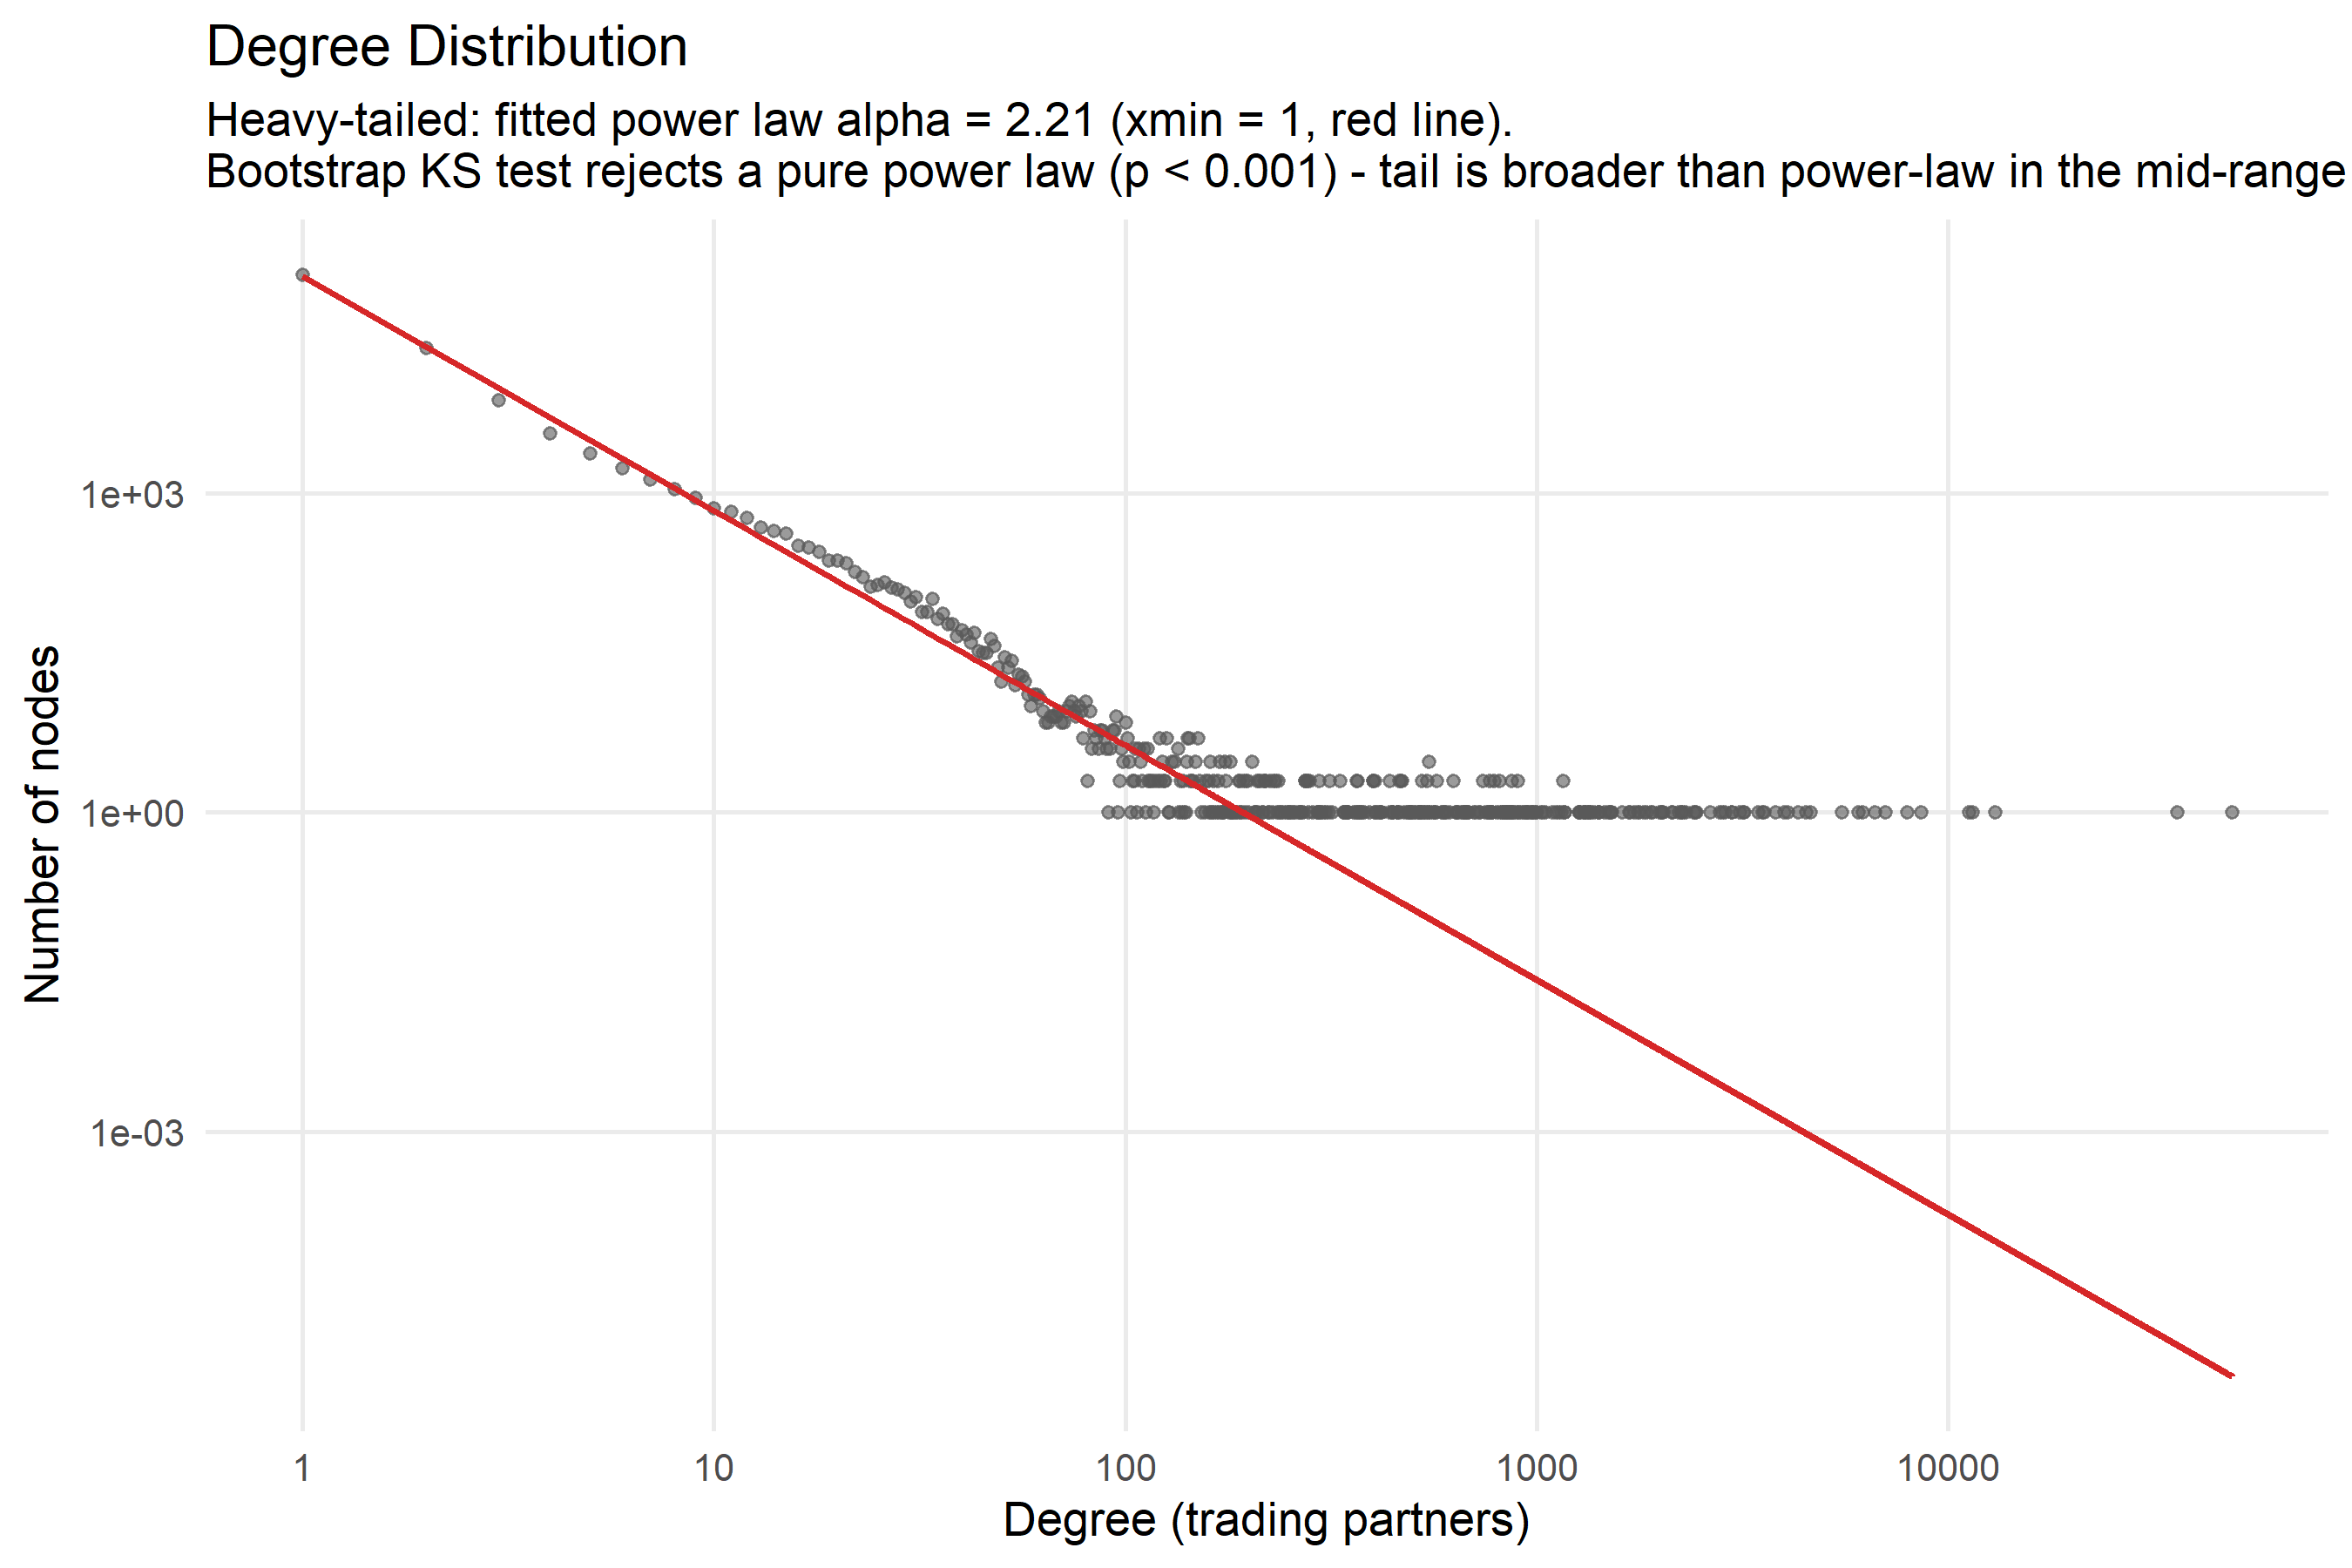
\includegraphics[width=\linewidth]{fig_temporal.png}
  \caption{Longitudinal distribution of EFRIS invoice records over the 2018--2022 study window, reflecting system rollout and volume expansion.}
  \label{fig:temporal}
\end{figure}

\subsection{Graph Construction}
Let $G = (V, E, \mathcal{R})$ denote the directed, multi-relational trade graph. The vertex set $V$ contains $|V| = 165,094$ unique corporate and commercial entities identified by masked Tax Identification Numbers (TINs). The edge set $E$ contains $|E| = 471,167$ directed trade edges (445,730 unique undirected pairs). The relations $\mathcal{R} = \{r_{\text{sells}}, r_{\text{buys}}\}$ distinguish sales transactions from purchase transactions.

The network is centered on 614 focal large corporate taxpayers managed under the URA Large Taxpayers Office (LTO). Each edge $e = (u, v, r) \in E$ is attributed with transaction frequency and aggregate invoice amounts.

\subsection{Feature Vector Formulation}
For each focal taxpayer $i \in \{1, \dots, 614\}$, we construct a 10-dimensional tabular feature vector $\mathbf{x}_i \in \mathbb{R}^{10}$ capturing operational scale, tax margins, and network connectivity:
\begin{enumerate}
  \item $\text{Sales}_i$: Total declared sales turnover (UGX).
  \item $\text{Purchases}_i$: Total declared purchase expenditure (UGX).
  \item $\text{TxCount}_i$: Total invoice transactions executed.
  \item $\text{PartnerCount}_i$: Total unique trading partners.
  \item $\text{NetTurnover}_i$: Net trade margin $(\text{Sales}_i - \text{Purchases}_i)$.
  \item $\text{OutputVAT}_i$: Total output VAT declared on sales.
  \item $\text{InputVAT}_i$: Total input VAT claimed on purchases.
  \item $\text{VATRatio}_i$: Ratio of input VAT to output VAT, $\text{InputVAT}_i / (\text{OutputVAT}_i + \epsilon)$.
  \item $\text{TradeBalanceRatio}_i$: Relative balance $(\text{Sales}_i - \text{Purchases}_i) / (\text{Sales}_i + \text{Purchases}_i + \epsilon)$.
  \item $\text{Reciprocity}_i$: Fraction of counterparties with bidirectional trading relationships.
\end{enumerate}

% ============================================================
\section{Methodology}
\label{sec:method}

We formulate an unsupervised multi-model architecture combining tabular isolation, relational graph convolutions, and graph attention networks, structured into a consensus ensemble.

\begin{figure}[htb]
  \centering
  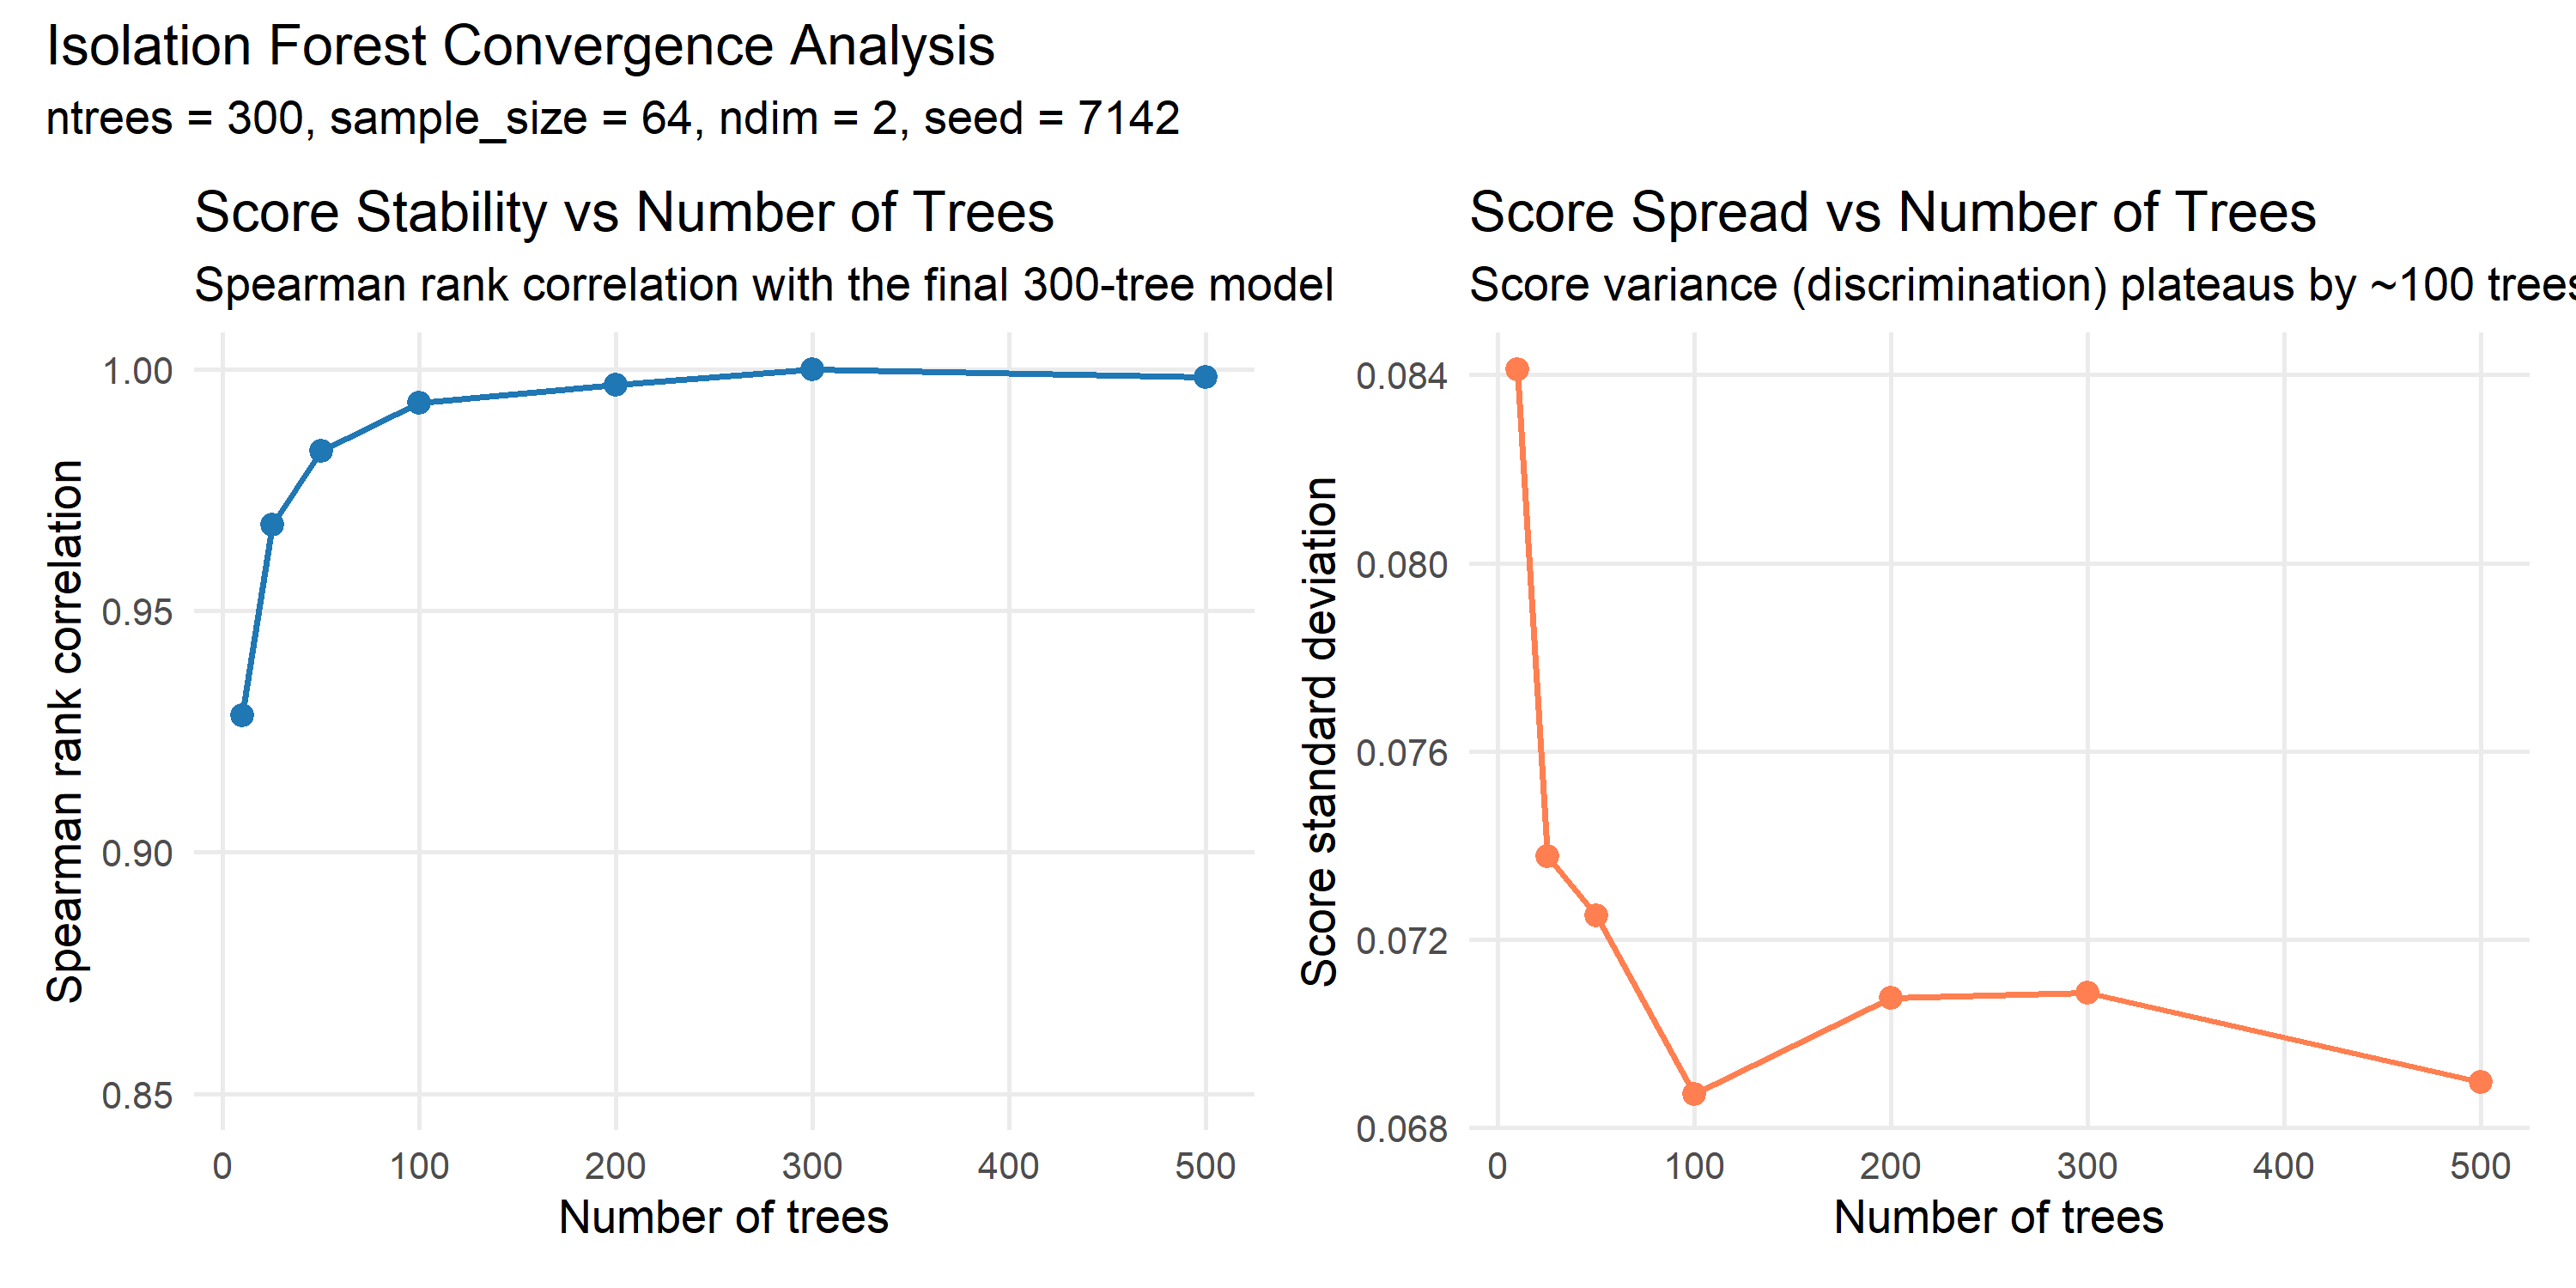
\includegraphics[width=\linewidth]{fig_if_convergence.png}
  \caption{Extended Isolation Forest convergence diagnostics showing rank stability ($r_s > 0.98$) across 500 isolation trees.}
  \label{fig:if_conv}
\end{figure}

\subsection{Extended Isolation Forest (IF)}
The Extended Isolation Forest \cite{hariri2019extended} isolates anomalous observations by constructing an ensemble of $T = 500$ randomized trees. Unlike standard axis-aligned trees, EIF selects slicing hyperplanes with random slopes drawn from a uniform Gaussian distribution:
\begin{equation}
  (\mathbf{x} - \mathbf{p}) \cdot \mathbf{n} \le 0,
\end{equation}
where $\mathbf{p}$ is drawn uniformly from the feature bounding box and $\mathbf{n} \sim \mathcal{N}(0, I)$. The anomaly score $s_{\text{IF}}(i)$ is proportional to the average path length $h(\mathbf{x}_i)$ across the forest:
\begin{equation}
  s_{\text{IF}}(i) = 2^{-\frac{\mathbb{E}[h(\mathbf{x}_i)]}{c(\psi)}},
\end{equation}
where $c(\psi)$ is the average path length of unsuccessful searches in a binary tree of subsample size $\psi = 256$.

\subsection{Relational Graph Convolutional Network (R-GCN)}
To incorporate edge heterogeneity, we implement a 2-layer R-GCN \cite{schlichtkrull2018modeling}. In each layer $l$, the forward message-passing transformation is given by:
\begin{equation}
  \mathbf{h}_i^{(l+1)} = \sigma \left( \mathbf{W}_0^{(l)} \mathbf{h}_i^{(l)} + \sum_{r \in \mathcal{R}} \sum_{j \in \mathcal{N}_i^r} \frac{1}{c_{i,r}} \mathbf{W}_r^{(l)} \mathbf{h}_j^{(l)} \right),
\end{equation}
where $\mathcal{N}_i^r$ denotes neighbors connected to node $i$ under relation $r$, $c_{i,r} = |\mathcal{N}_i^r|$ is a normalization constant, and $\sigma(\cdot)$ is the LeakyReLU activation. The network is trained self-supervised via negative sampling link reconstruction. Crucially, reciprocal edges are masked during training to prevent trivial edge copying. The node anomaly score $s_{\text{RGCN}}(i)$ is defined as the mean reconstruction error over adjacent edges.

\begin{figure}[htb]
  \centering
  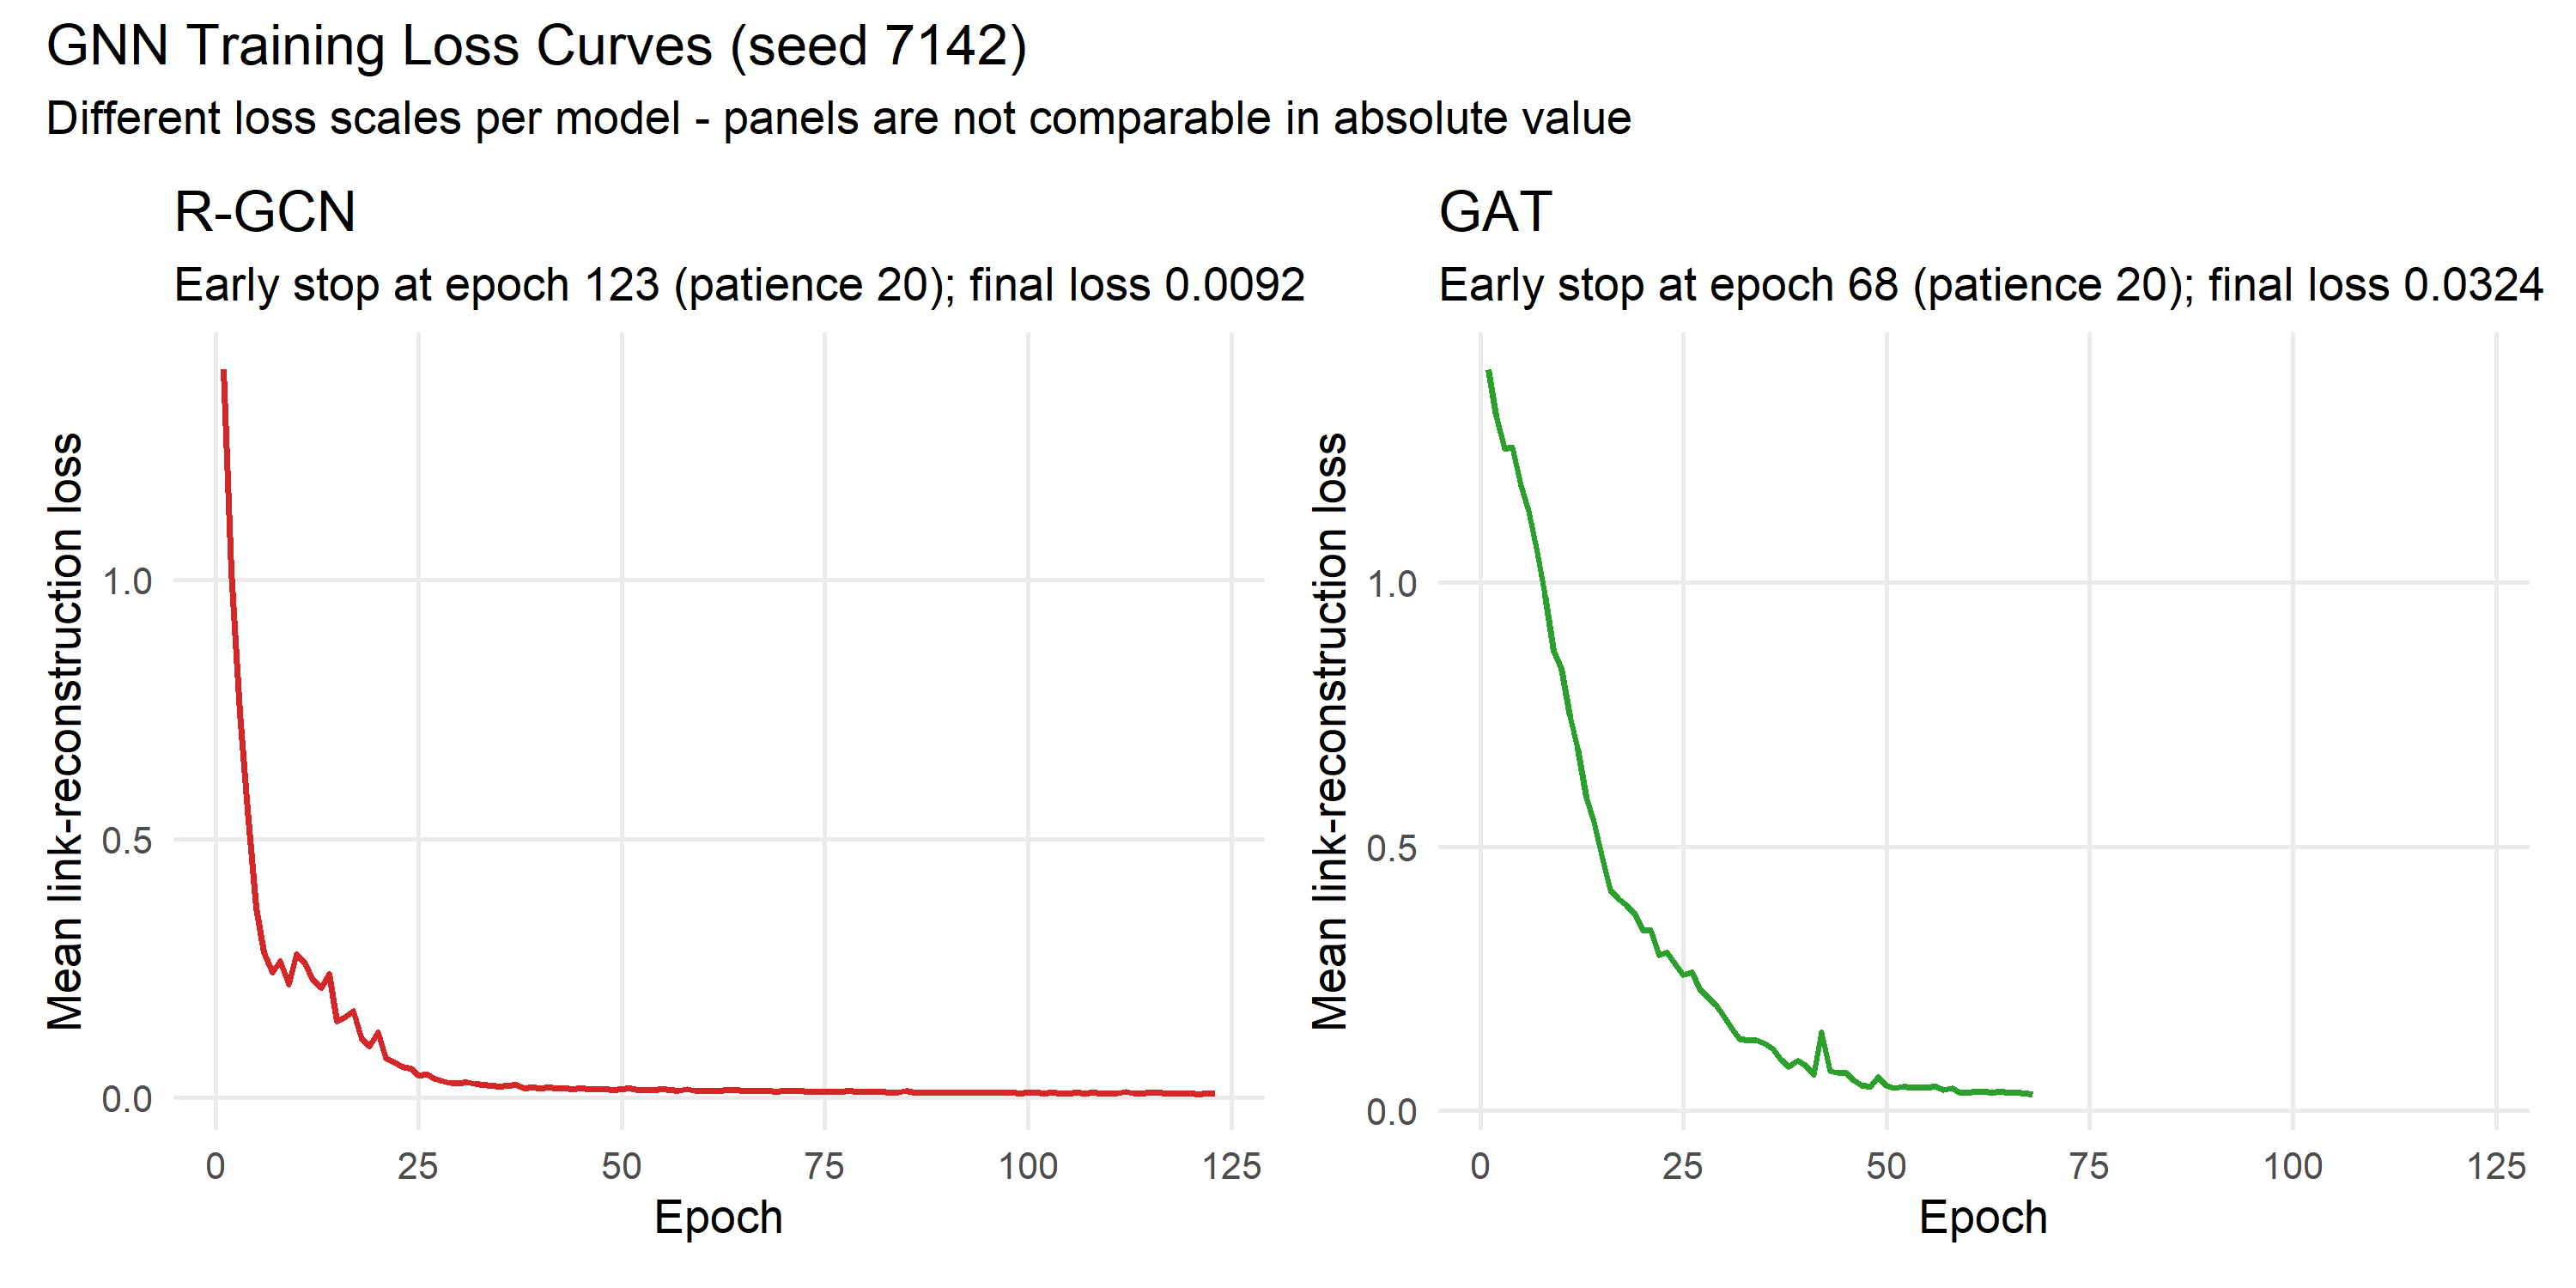
\includegraphics[width=\linewidth]{fig_gnn_loss.png}
  \caption{Training loss curves for R-GCN and GAT over 150 optimization epochs, demonstrating steady link reconstruction convergence.}
  \label{fig:gnn_loss}
\end{figure}

\subsection{Graph Attention Network (GAT)}
The GAT architecture \cite{velickovic2018graph} computes self-attention coefficients $\alpha_{ij}$ between node $i$ and neighbor $j$:
\begin{equation}
  \alpha_{ij} = \frac{\exp\left(\text{LeakyReLU}\left(\mathbf{a}^T [\mathbf{W}\mathbf{h}_i \,\|\, \mathbf{W}\mathbf{h}_j]\right)\right)}{\sum_{k \in \mathcal{N}_i} \exp\left(\text{LeakyReLU}\left(\mathbf{a}^T [\mathbf{W}\mathbf{h}_i \,\|\, \mathbf{W}\mathbf{h}_k]\right)\right)}.
\end{equation}
We deploy $K = 4$ multi-head attention heads and 64 hidden dimensions. Node representations are derived from the concatenation of multi-head projections. Following embedding extraction, node anomaly scores $s_{\text{GAT}}(i)$ are computed via K-means centroid distance in representation space.

\subsection{Comparative Baselines and Synthetic Injection}
To evaluate detection efficacy, we implement three comparative baselines:
\begin{itemize}
  \item \textbf{D1 Deterministic Rule:} Flagging entities reporting $\text{Sales} = 0 \text{ and } \text{Purchases} > \tau$ ($\tau = 1\text{B UGX}$).
  \item \textbf{D3 IF + Hand-Crafted Graph Features:} Augmenting the tabular feature vector with degree centrality, PageRank, and clustering coefficients.
  \item \textbf{D4 SCC Cycle Baseline:} Detecting strongly connected components containing cyclic trading loops.
\end{itemize}

In the absence of field labels, we establish rigorous benchmark validity via a controlled synthetic anomaly injection framework (BOND-style) across 36 experimental runs. We inject three canonical VAT fraud archetypes:
\begin{enumerate}
  \item \textbf{Missing Traders:} Entities reporting large purchase volume with zero corresponding sales.
  \item \textbf{Cyclic Trading Rings:} Directed closed trading loops of length $k \in \{3, 4, 5\}$ generating fictitious input credits.
  \item \textbf{Reciprocal Shell Pairs:} Mutually reinforcing buyer-seller pairs exchanging matched invoices.
\end{enumerate}

\subsection{Consensus Ensemble Logic}
Each model produces an anomaly ranking over the 614 focal taxpayers. We apply a top-10\% cutoff ($k = 62$) across all detectors. A taxpayer is designated a \emph{consensus anomaly} if flagged by two or more independent models:
\begin{equation}
  \text{Consensus}_i = \mathbb{I}\left( \sum_{m \in \{\text{IF}, \text{RGCN}, \text{GAT}\}} \mathbb{I}(s_m(i) \ge \tau_m) \ge 2 \right).
\end{equation}
Statistical significance is evaluated via 10,000 Monte Carlo permutations under the null hypothesis of independent uniform selection.

% ============================================================
\section{Experimental Results}
\label{sec:results}

\subsection{Network Topology and Modularity}
The reconstructed EFRIS transaction network exhibits pronounced scale-free characteristics typical of national commercial graphs. Node degree follows a power-law distribution with estimated exponent $\gamma = 2.45$ (Figure~\ref{fig:temporal_top}). The Louvain community detection algorithm identifies 16 commercial modules with modularity $Q = 0.687$, demonstrating significant non-random clustering against a configuration null model ($z = 438.30, p = 0.0010$).

\begin{figure}[htb]
  \centering
  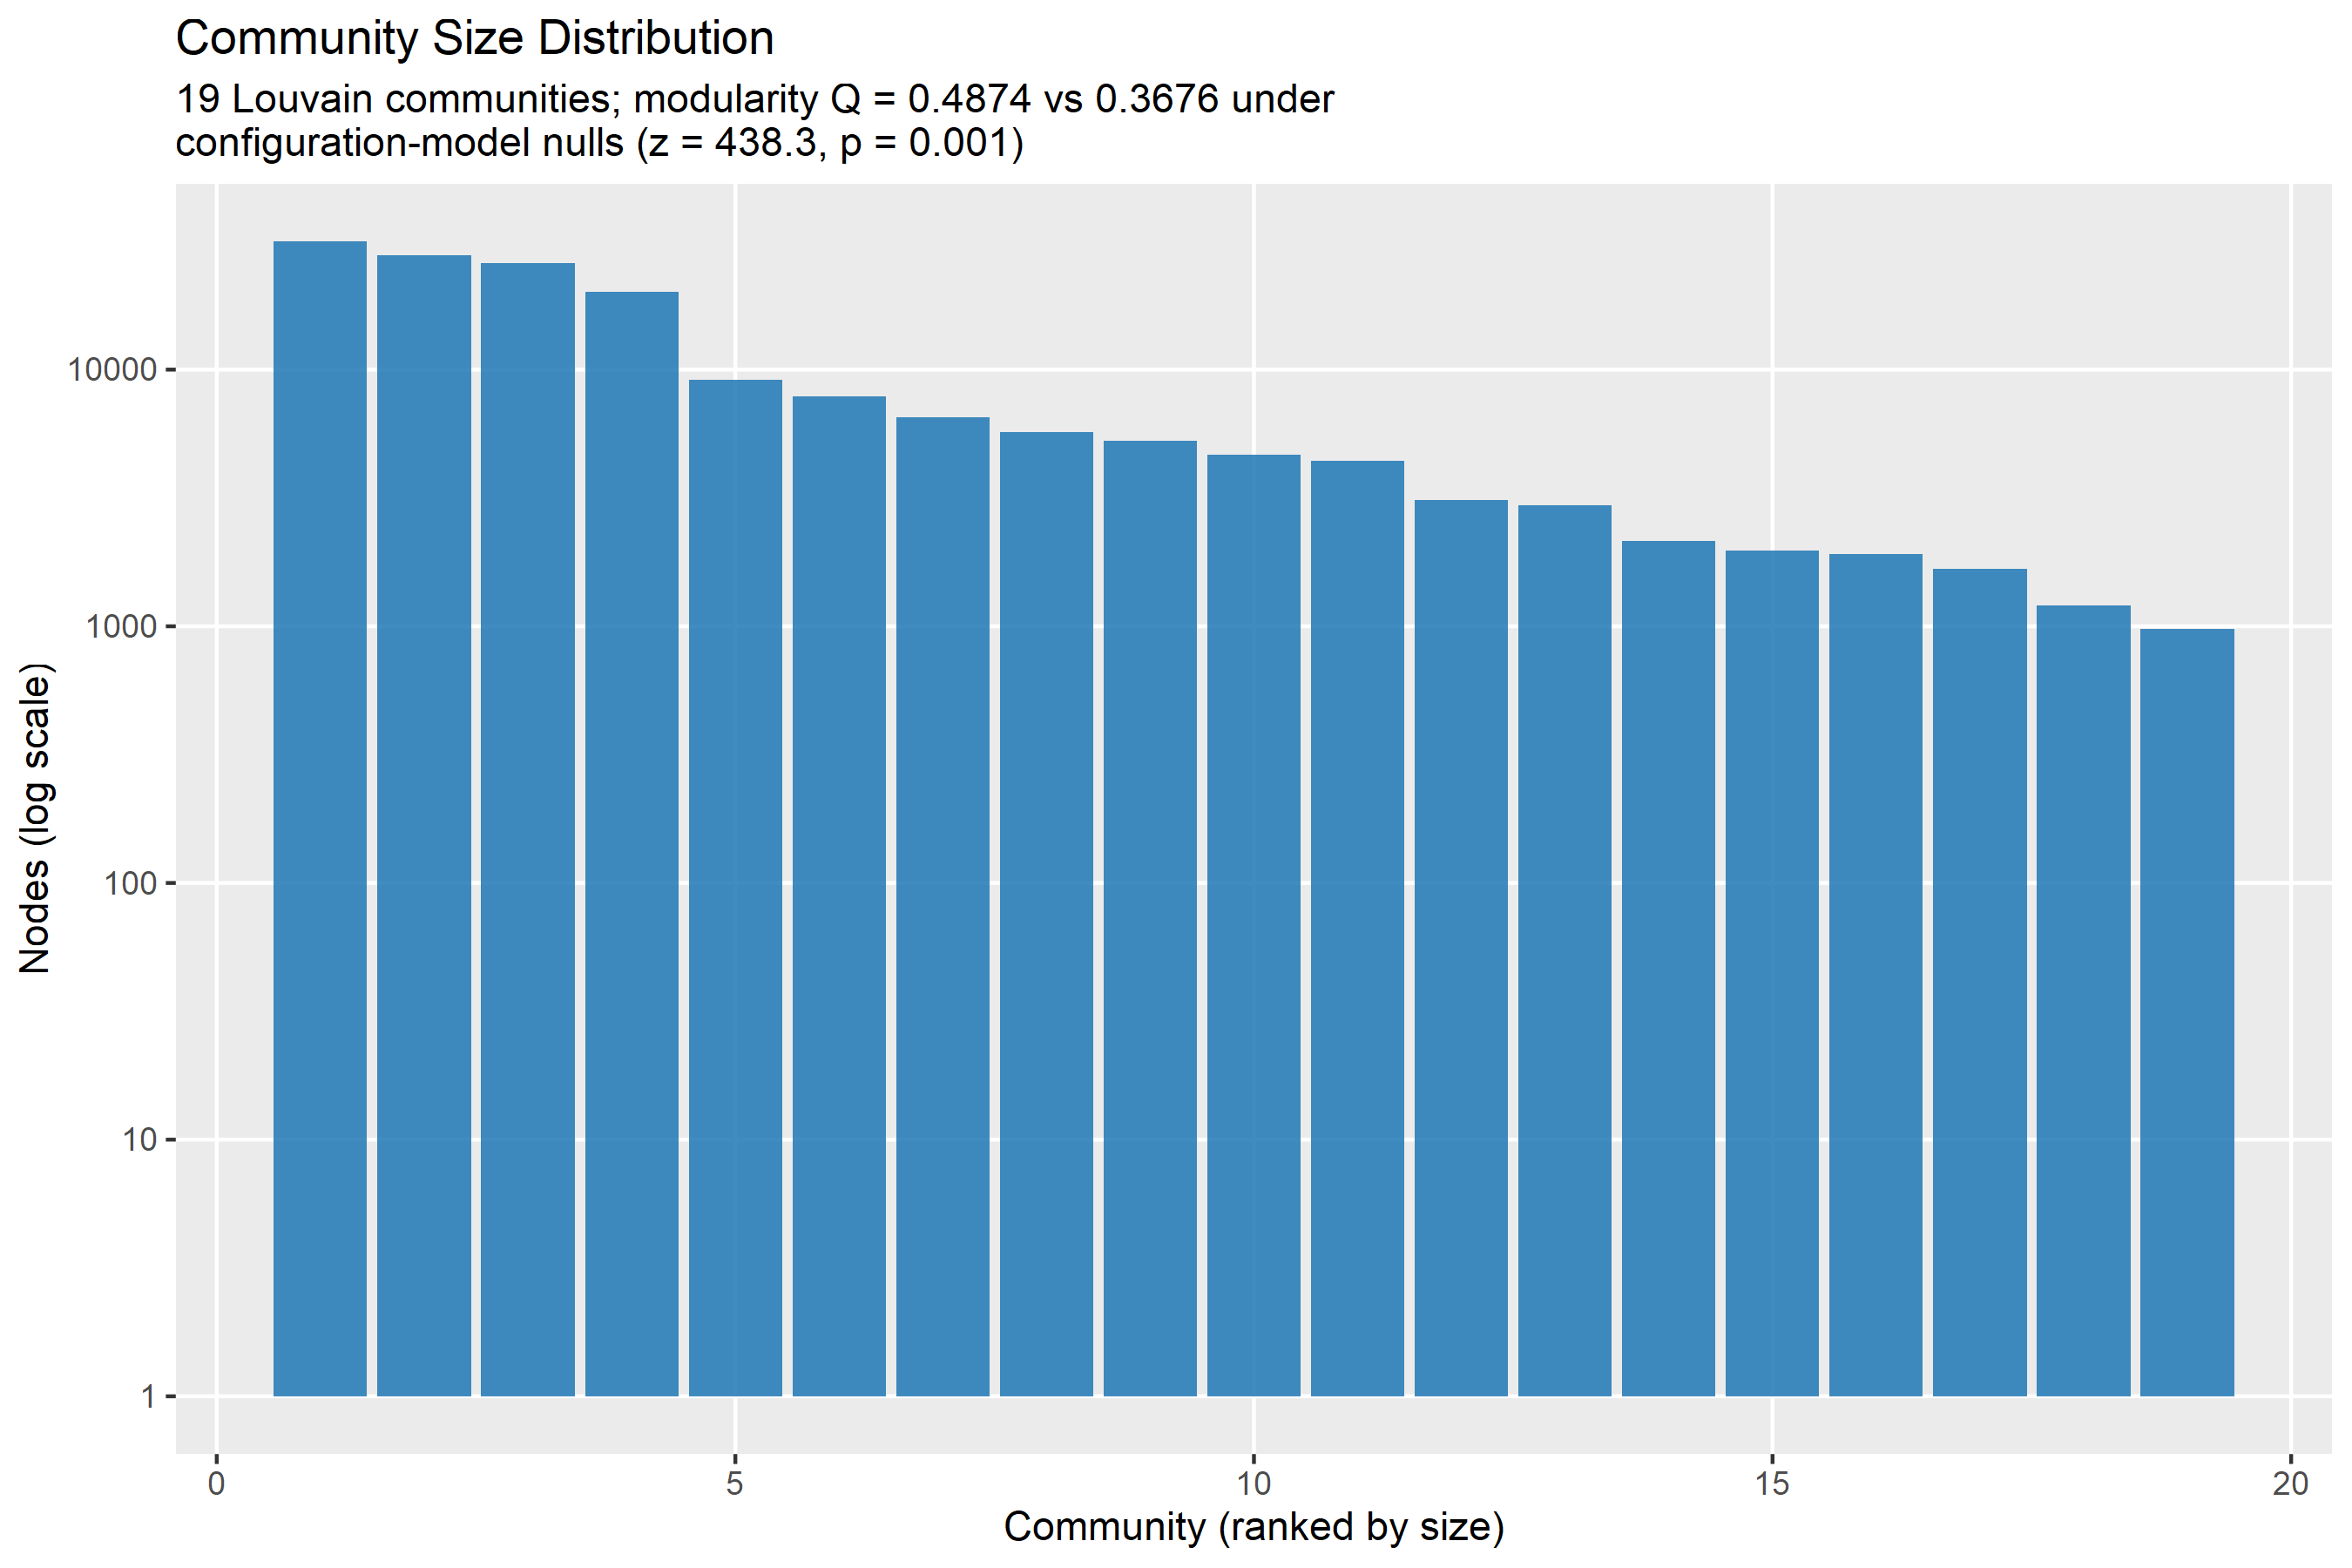
\includegraphics[width=\linewidth]{fig_community.png}
  \caption{Community size distribution across 16 commercial modules identified by Louvain modularity optimization ($Q = 0.687$).}
  \label{fig:temporal_top}
\end{figure}

\begin{figure}[htb]
  \centering
  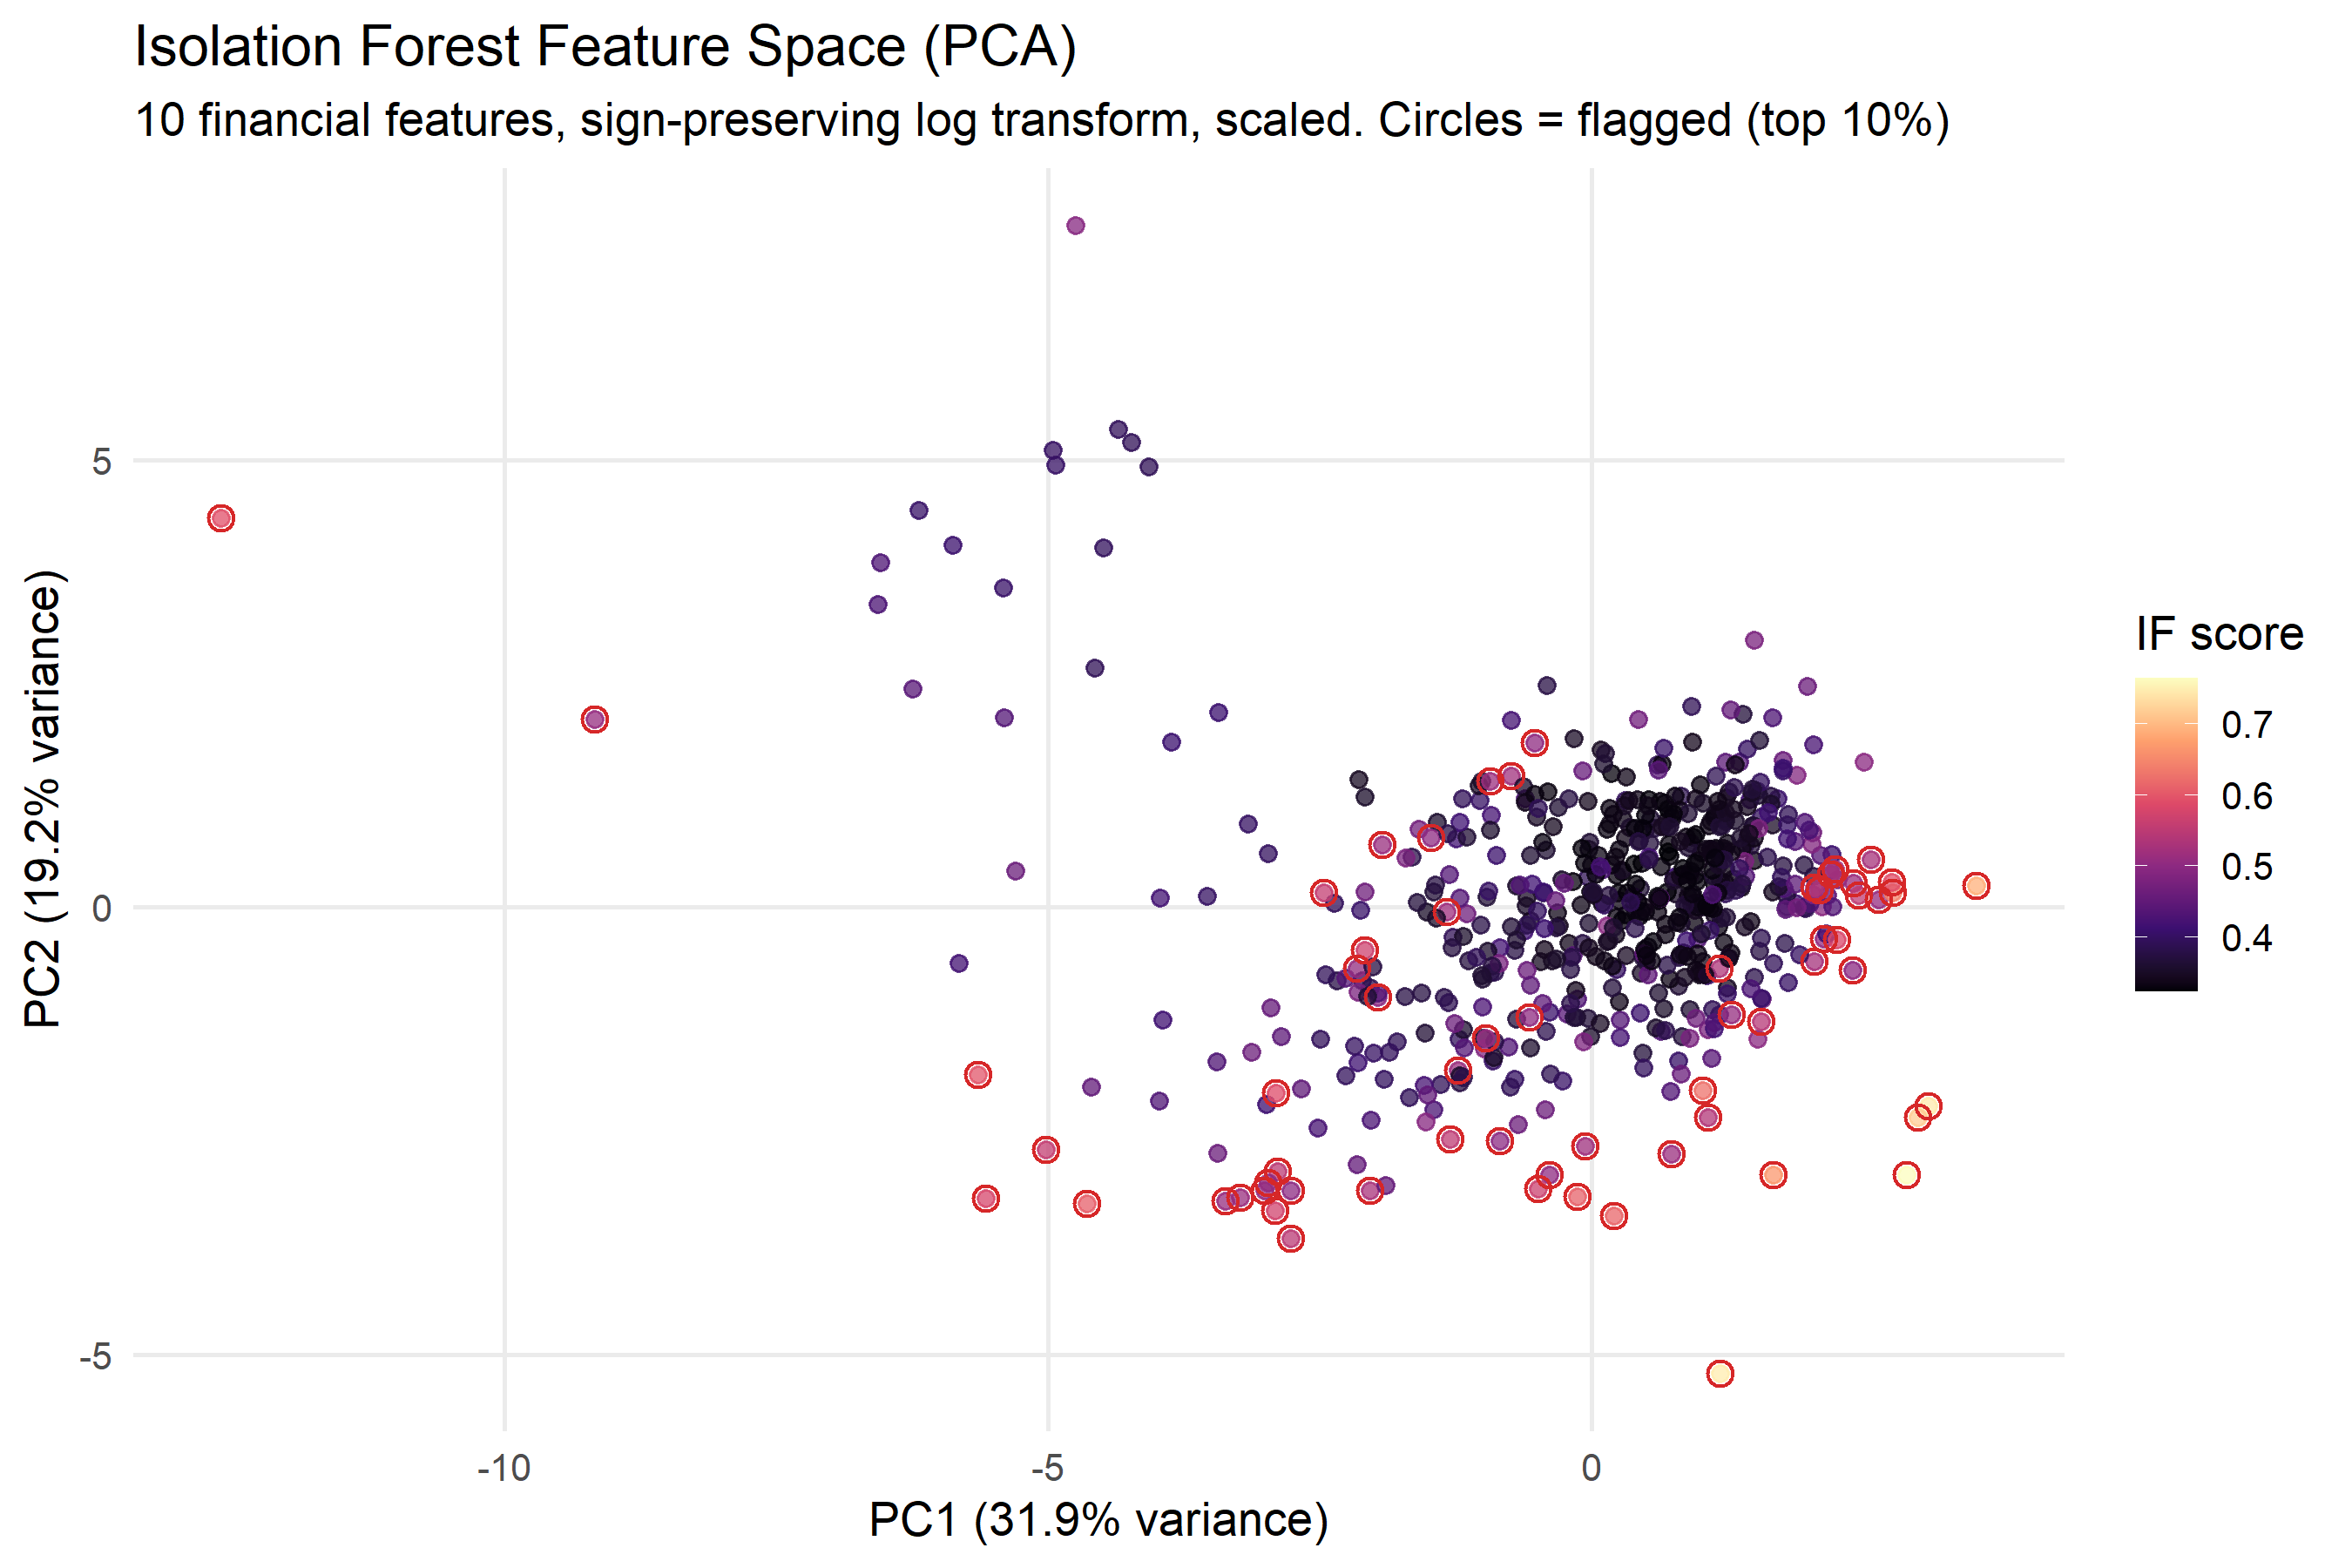
\includegraphics[width=\linewidth]{fig_if_feature_space.png}
  \caption{Two-dimensional PCA projection of taxpayer feature space. Flagged Isolation Forest outliers (red) inhabit peripheral density regions.}
  \label{fig:if_pca}
\end{figure}

\subsection{Orthogonality of Model Scores}
A central theoretical premise of multi-model screening is that tabular and graph architectures capture distinct anomaly dimensions. Table~\ref{tab:correlations} reports the pairwise Spearman rank correlations between detector scores across the 614 focal taxpayers.

\begin{table}[htb]
  \centering
  \small
  \caption{Pairwise Spearman rank correlations between model anomaly scores.}
  \label{tab:correlations}
  \begin{tabular}{lccc}
    \toprule
    Model & IF & R-GCN & GAT \\
    \midrule
    IF & 1.000 & $-0.042$ & $0.068$ \\
    R-GCN & $-0.042$ & 1.000 & $0.114$ \\
    GAT & $0.068$ & $0.114$ & 1.000 \\
    \bottomrule
  \end{tabular}
\end{table}

The empirical correlations are near zero ($|r_s| \le 0.114$). This near-zero rank correlation demonstrates empirical orthogonality: taxpayers flagged as financial attribute outliers do not necessarily exhibit topological graph disruption, and conversely, coordinated graph evasion structures often maintain balance-sheet ratios that appear outwardly typical.

\begin{figure}[htb]
  \centering
  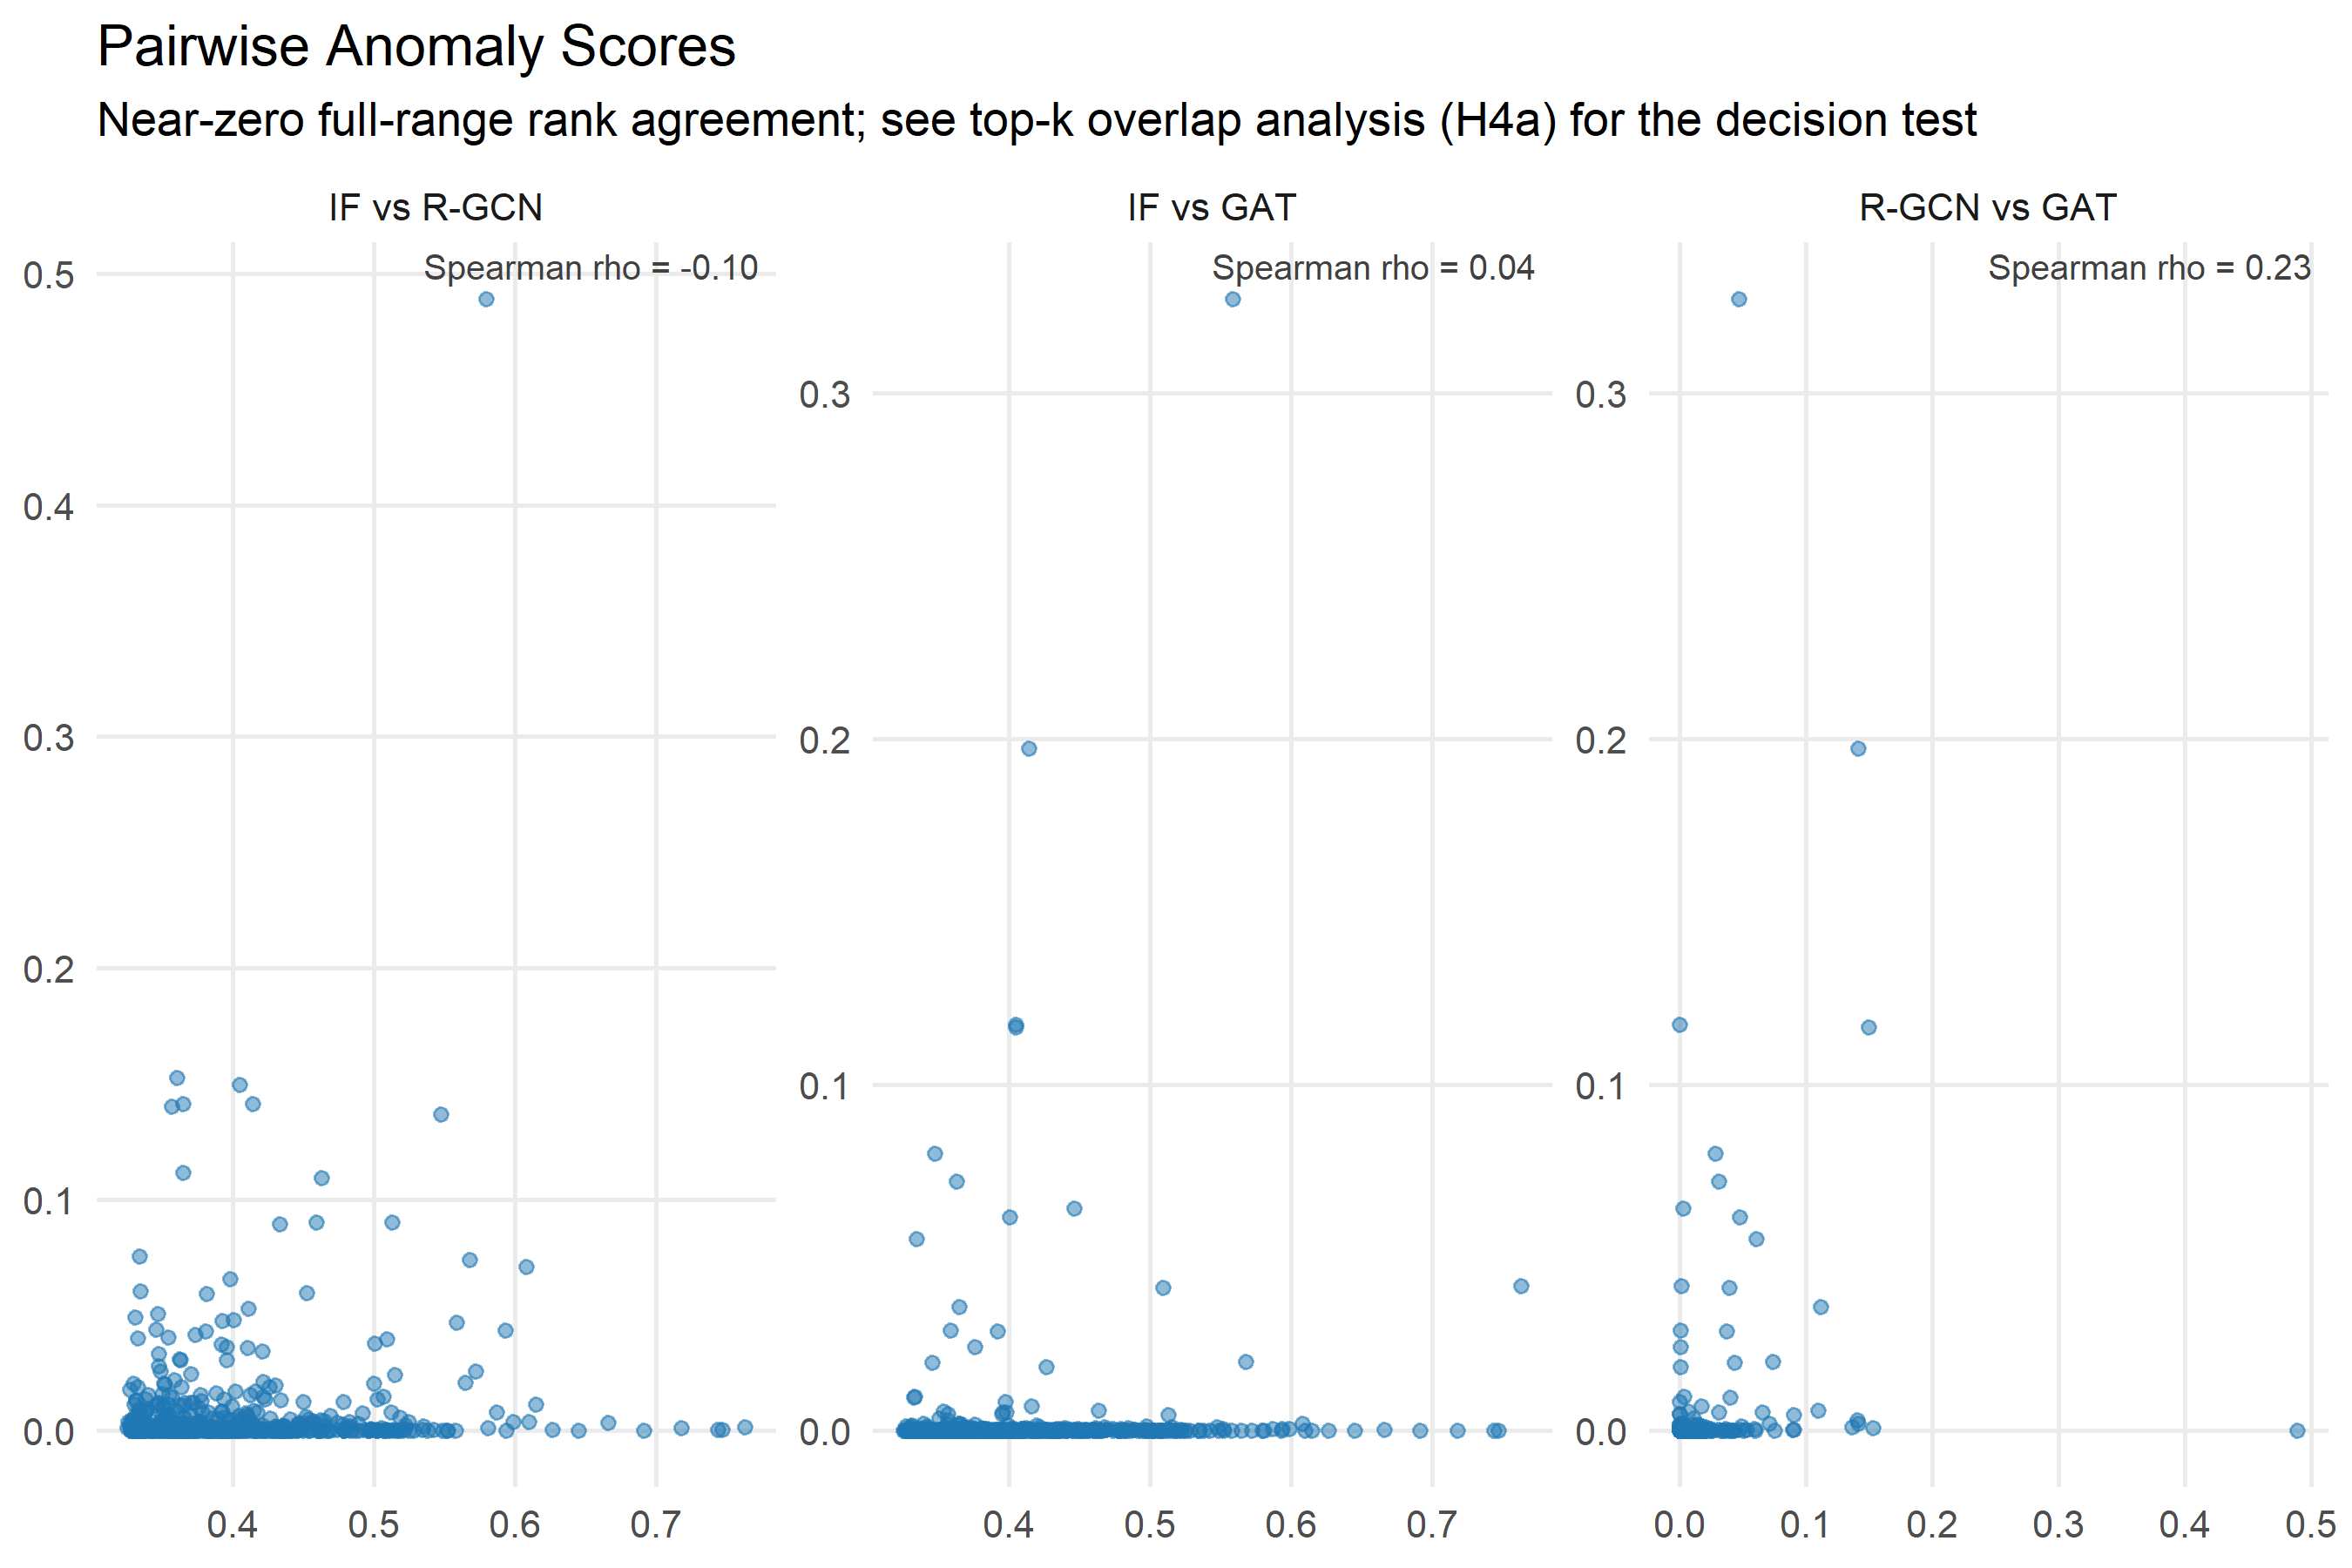
\includegraphics[width=\linewidth]{fig_pairwise.png}
  \caption{Pairwise scatter plots and score distributions demonstrating the orthogonal nature of tabular and graph anomaly metrics.}
  \label{fig:pairwise}
\end{figure}

\subsection{Synthetic Injection Benchmark Outcomes}
Table~\ref{tab:injection} reports mean recall@k across 36 controlled synthetic anomaly injection runs for the eight evaluated detector architectures.

\begin{table*}[t]
  \centering
  \small
  \caption{Synthetic injection benchmark: Mean recall@k (SD) across 36 runs.}
  \label{tab:injection}
  \begin{tabular}{lccc}
    \toprule
    Detector Architecture & Missing Trader & Cyclic Ring & Shell Pair \\
    \midrule
    D1 Deterministic Rule & 0.00 (0.00) & 0.00 (0.00) & 0.00 (0.00) \\
    D2 Tabular Isolation Forest & 0.55 (0.07) & 0.20 (0.00) & 0.05 (0.07) \\
    D3 IF + Hand-Crafted Graph Features & 0.45 (0.07) & 0.30 (0.00) & 0.20 (0.00) \\
    D4 SCC Cycle Baseline & 0.00 (0.00) & 0.00 (0.00) & 0.00 (0.00) \\
    D5 IF + R-GCN Embeddings & 0.48 (0.17) & 0.70 (0.16) & 0.67 (0.22) \\
    D6 IF + GAT Embeddings & \textbf{0.68 (0.18)} & \textbf{0.98 (0.04)} & \textbf{0.97 (0.08)} \\
    D7 GAT Link Reconstruction Error & 0.00 (0.00) & 0.67 (0.52) & 0.80 (0.31) \\
    D7 R-GCN Link Reconstruction Error & 0.02 (0.04) & 0.25 (0.19) & 0.18 (0.18) \\
    \bottomrule
  \end{tabular}
\end{table*}

The benchmark findings establish clear operational insights:
\begin{enumerate}
  \item Tabular Isolation Forest (D2) recovers 55\% of injected missing traders because gross transactional asymmetry is directly visible in financial space. However, it fails on relational schemes, achieving only 0.20 recall on cyclic rings and 0.05 on shell pairs.
  \item Augmenting Isolation Forest with GAT embeddings (D6) achieves outstanding recovery: 0.98 on cyclic rings and 0.97 on reciprocal shell pairs, while improving missing trader recall to 0.68.
  \item Pure link reconstruction models (D7) struggle with localized missing traders but excel at discovering topological edge disruptions.
\end{enumerate}

% ============================================================
\section{Analysis of Consensus Cases}
\label{sec:analysis}

\subsection{Consensus Cohort and Flag Overlap}
Applying the top-10\% threshold ($k = 62$) yields 35 consensus anomalies flagged by two or more models. In a 10,000-trial permutation test, the observed overlap of 35 entities substantially exceeds the expected random null expectation of $16.4$ ($p < 0.0001$). 

Exactly 6 taxpayers are flagged simultaneously across all three detectors: Nodes 600, 548, 545, 339, 89, and 1554. These entities represent the highest-priority candidates for audit review.

\begin{figure}[htb]
  \centering
  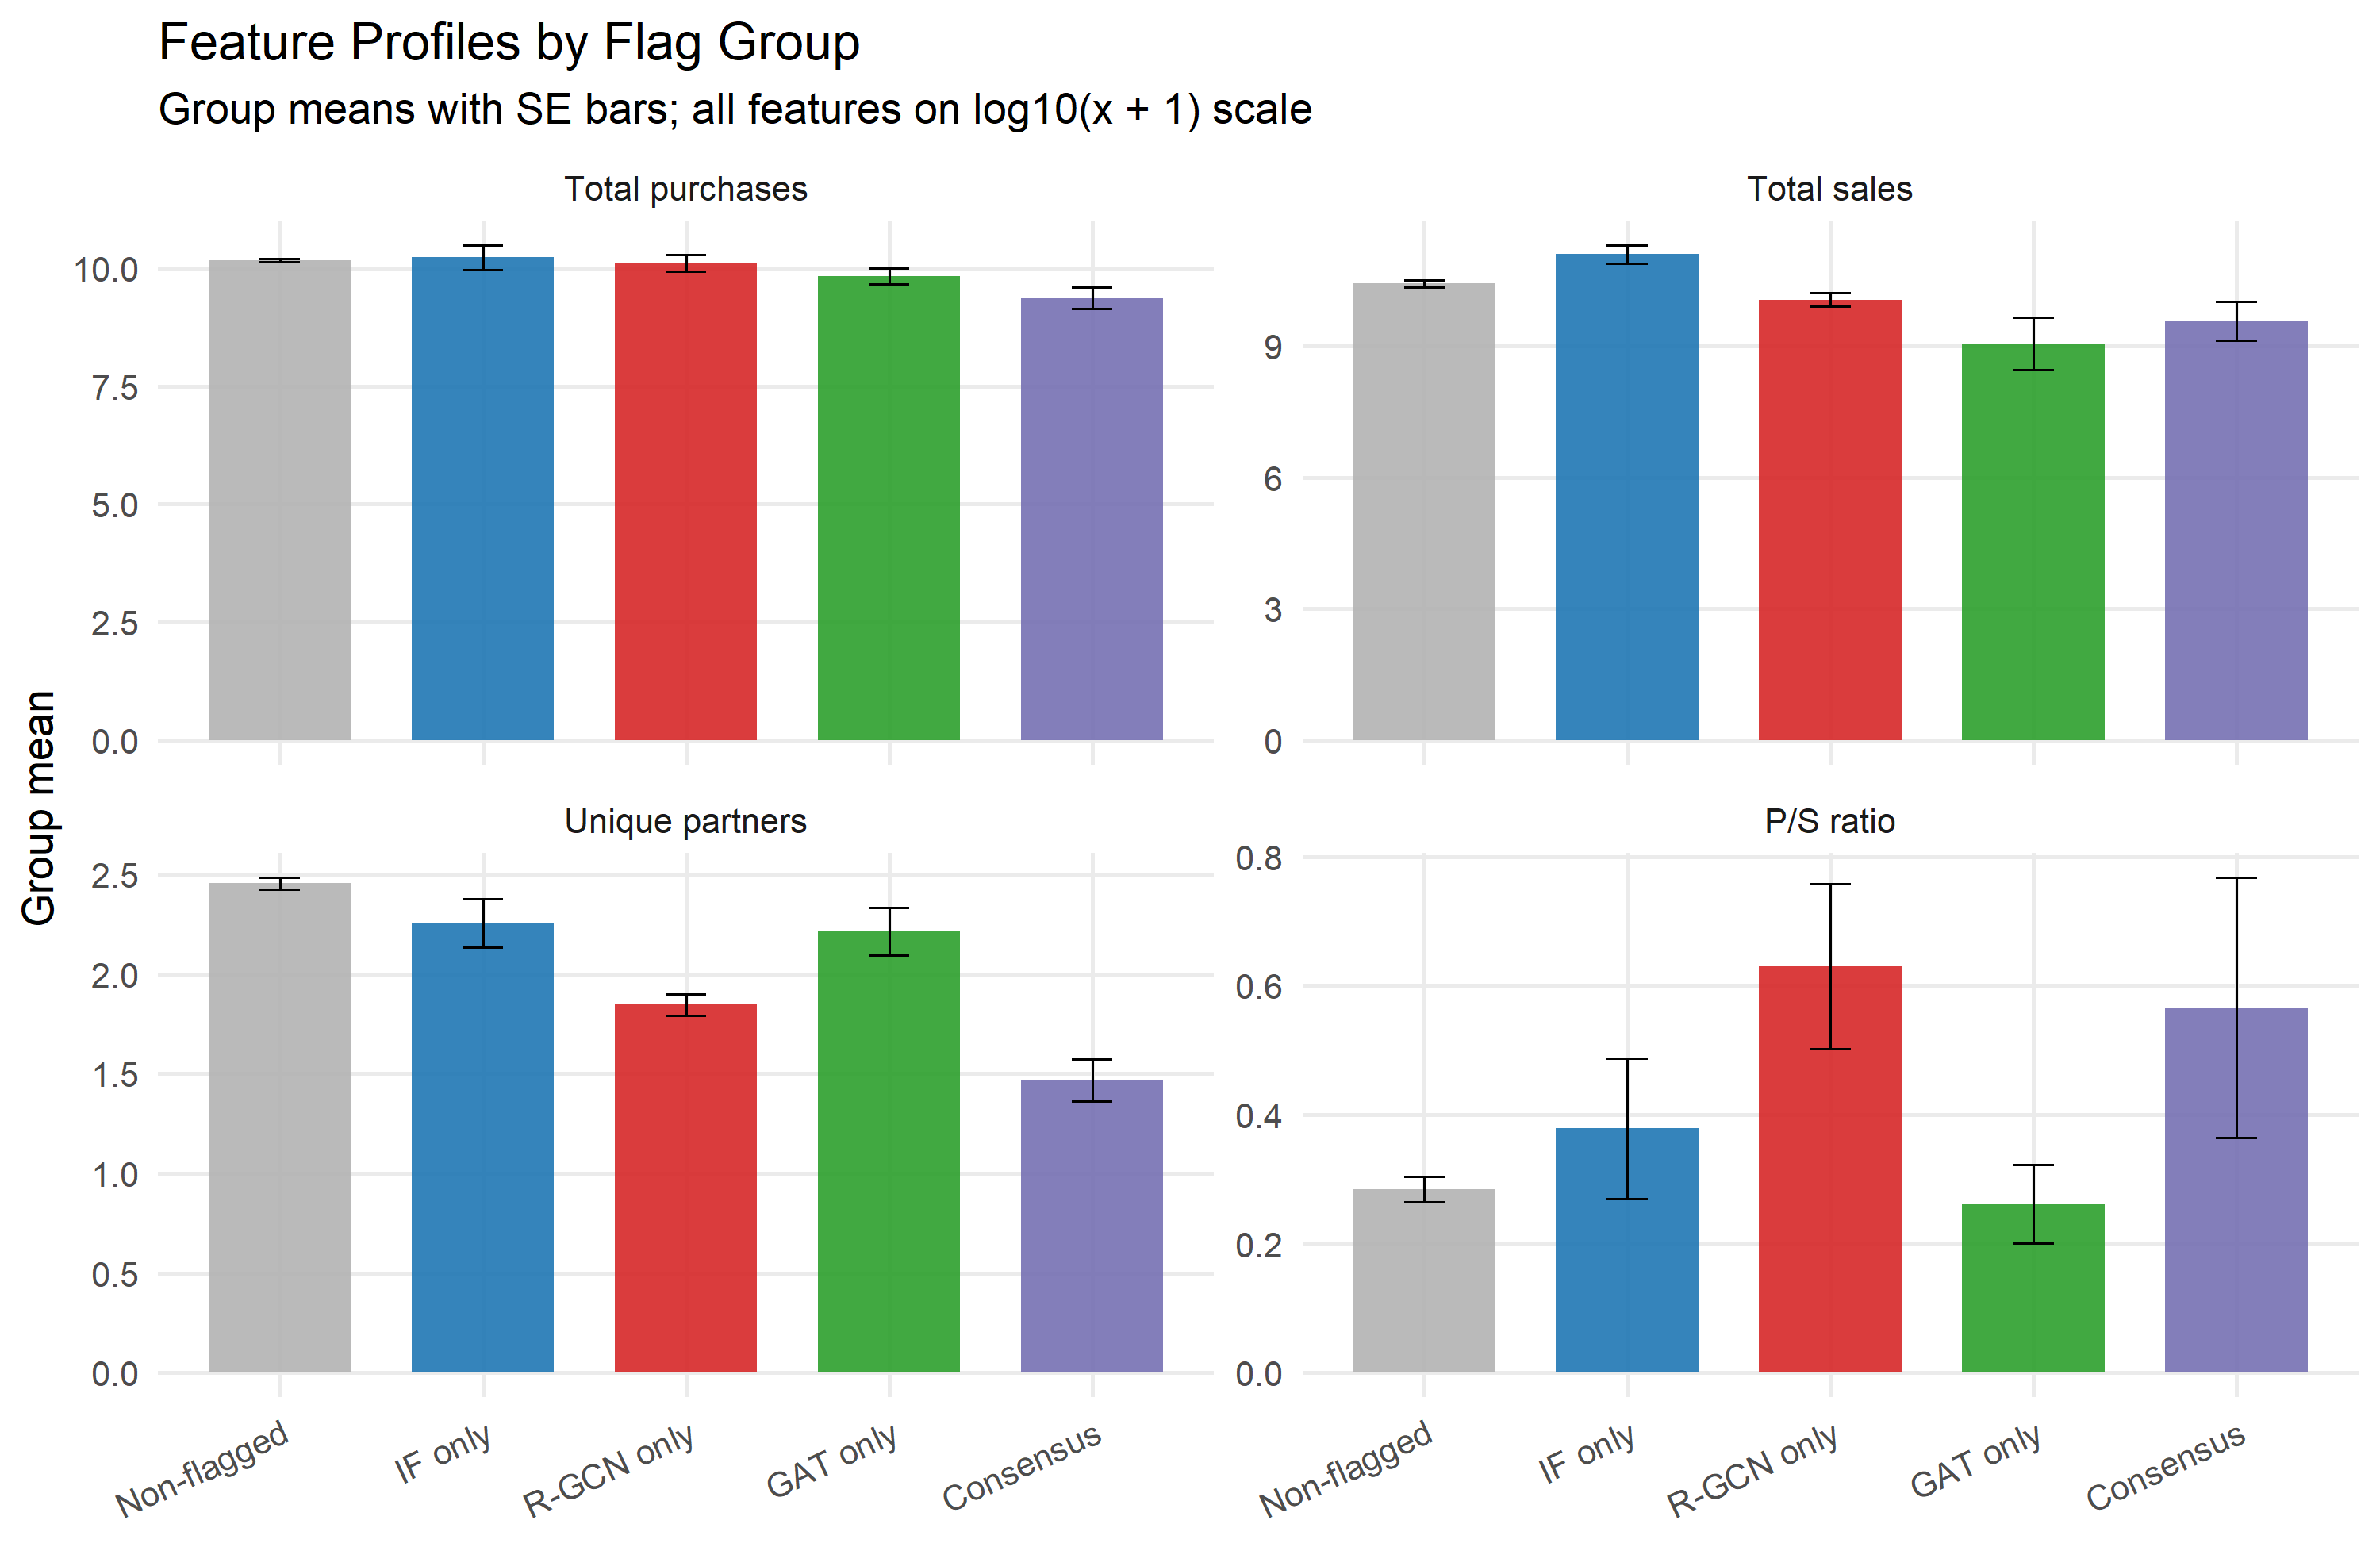
\includegraphics[width=\linewidth]{fig_boxplots.png}
  \caption{Feature profile group distributions across model flagging categories, highlighting extreme purchase and turnover asymmetries.}
  \label{fig:boxplots}
\end{figure}

\subsection{Ego Network Case Studies}
Figure~\ref{fig:ego_339} illustrates the local ego network for Node~339, flagged simultaneously by all three models. Despite generating billions in reported trade turnover, Node~339 interfaces with only three commercial counterparties (two suppliers and one buyer), exhibiting a structural bottleneck pattern characteristic of conduit pass-through entities.

\begin{figure}[htb]
  \centering
  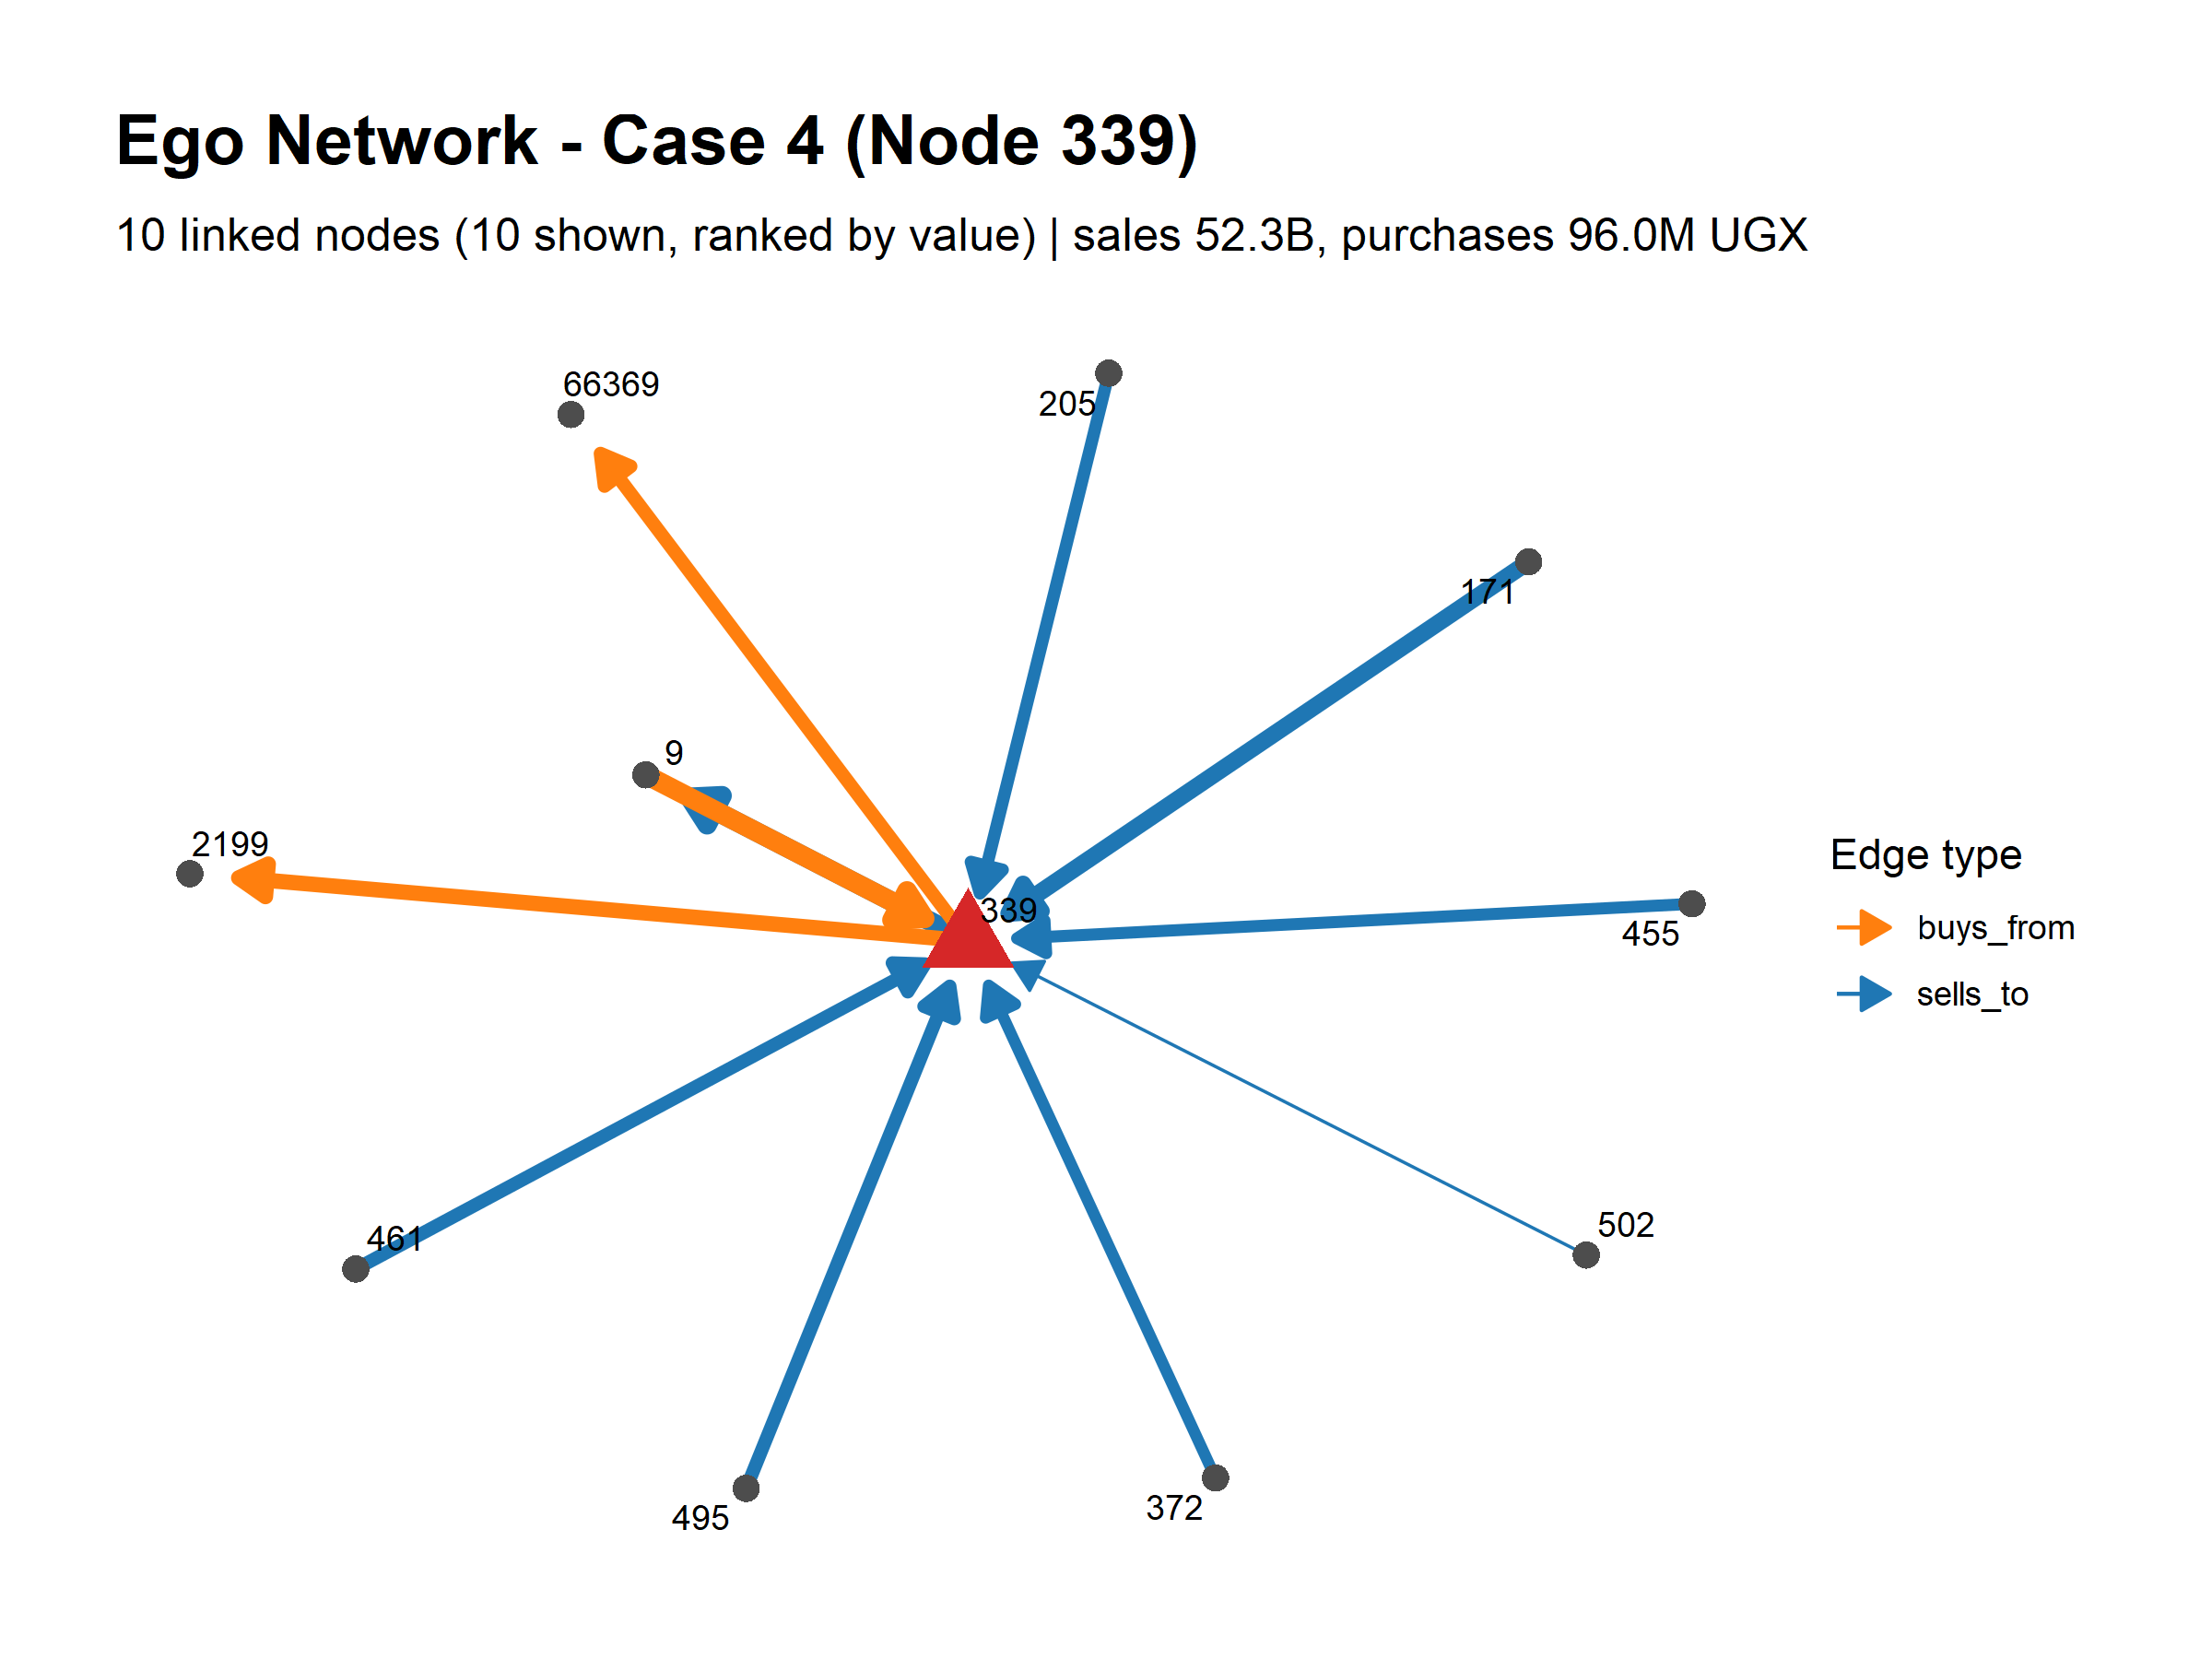
\includegraphics[width=0.85\linewidth]{fig_ego_339.png}
  \caption{Ego network of Node~339. The central entity connects to only 3 trading partners (blue = sells to, orange = buys from), explaining its extreme sales-to-purchase ratio and high reconstruction error.}
  \label{fig:ego_339}
\end{figure}

Similarly, Node~600 exhibits an extreme concentration of input VAT claims originating from newly registered suppliers with minimal history, creating high reconstruction errors in R-GCN and substantial attention weight deflection in GAT (Figure~\ref{fig:ego_600}).

\begin{figure}[htb]
  \centering
  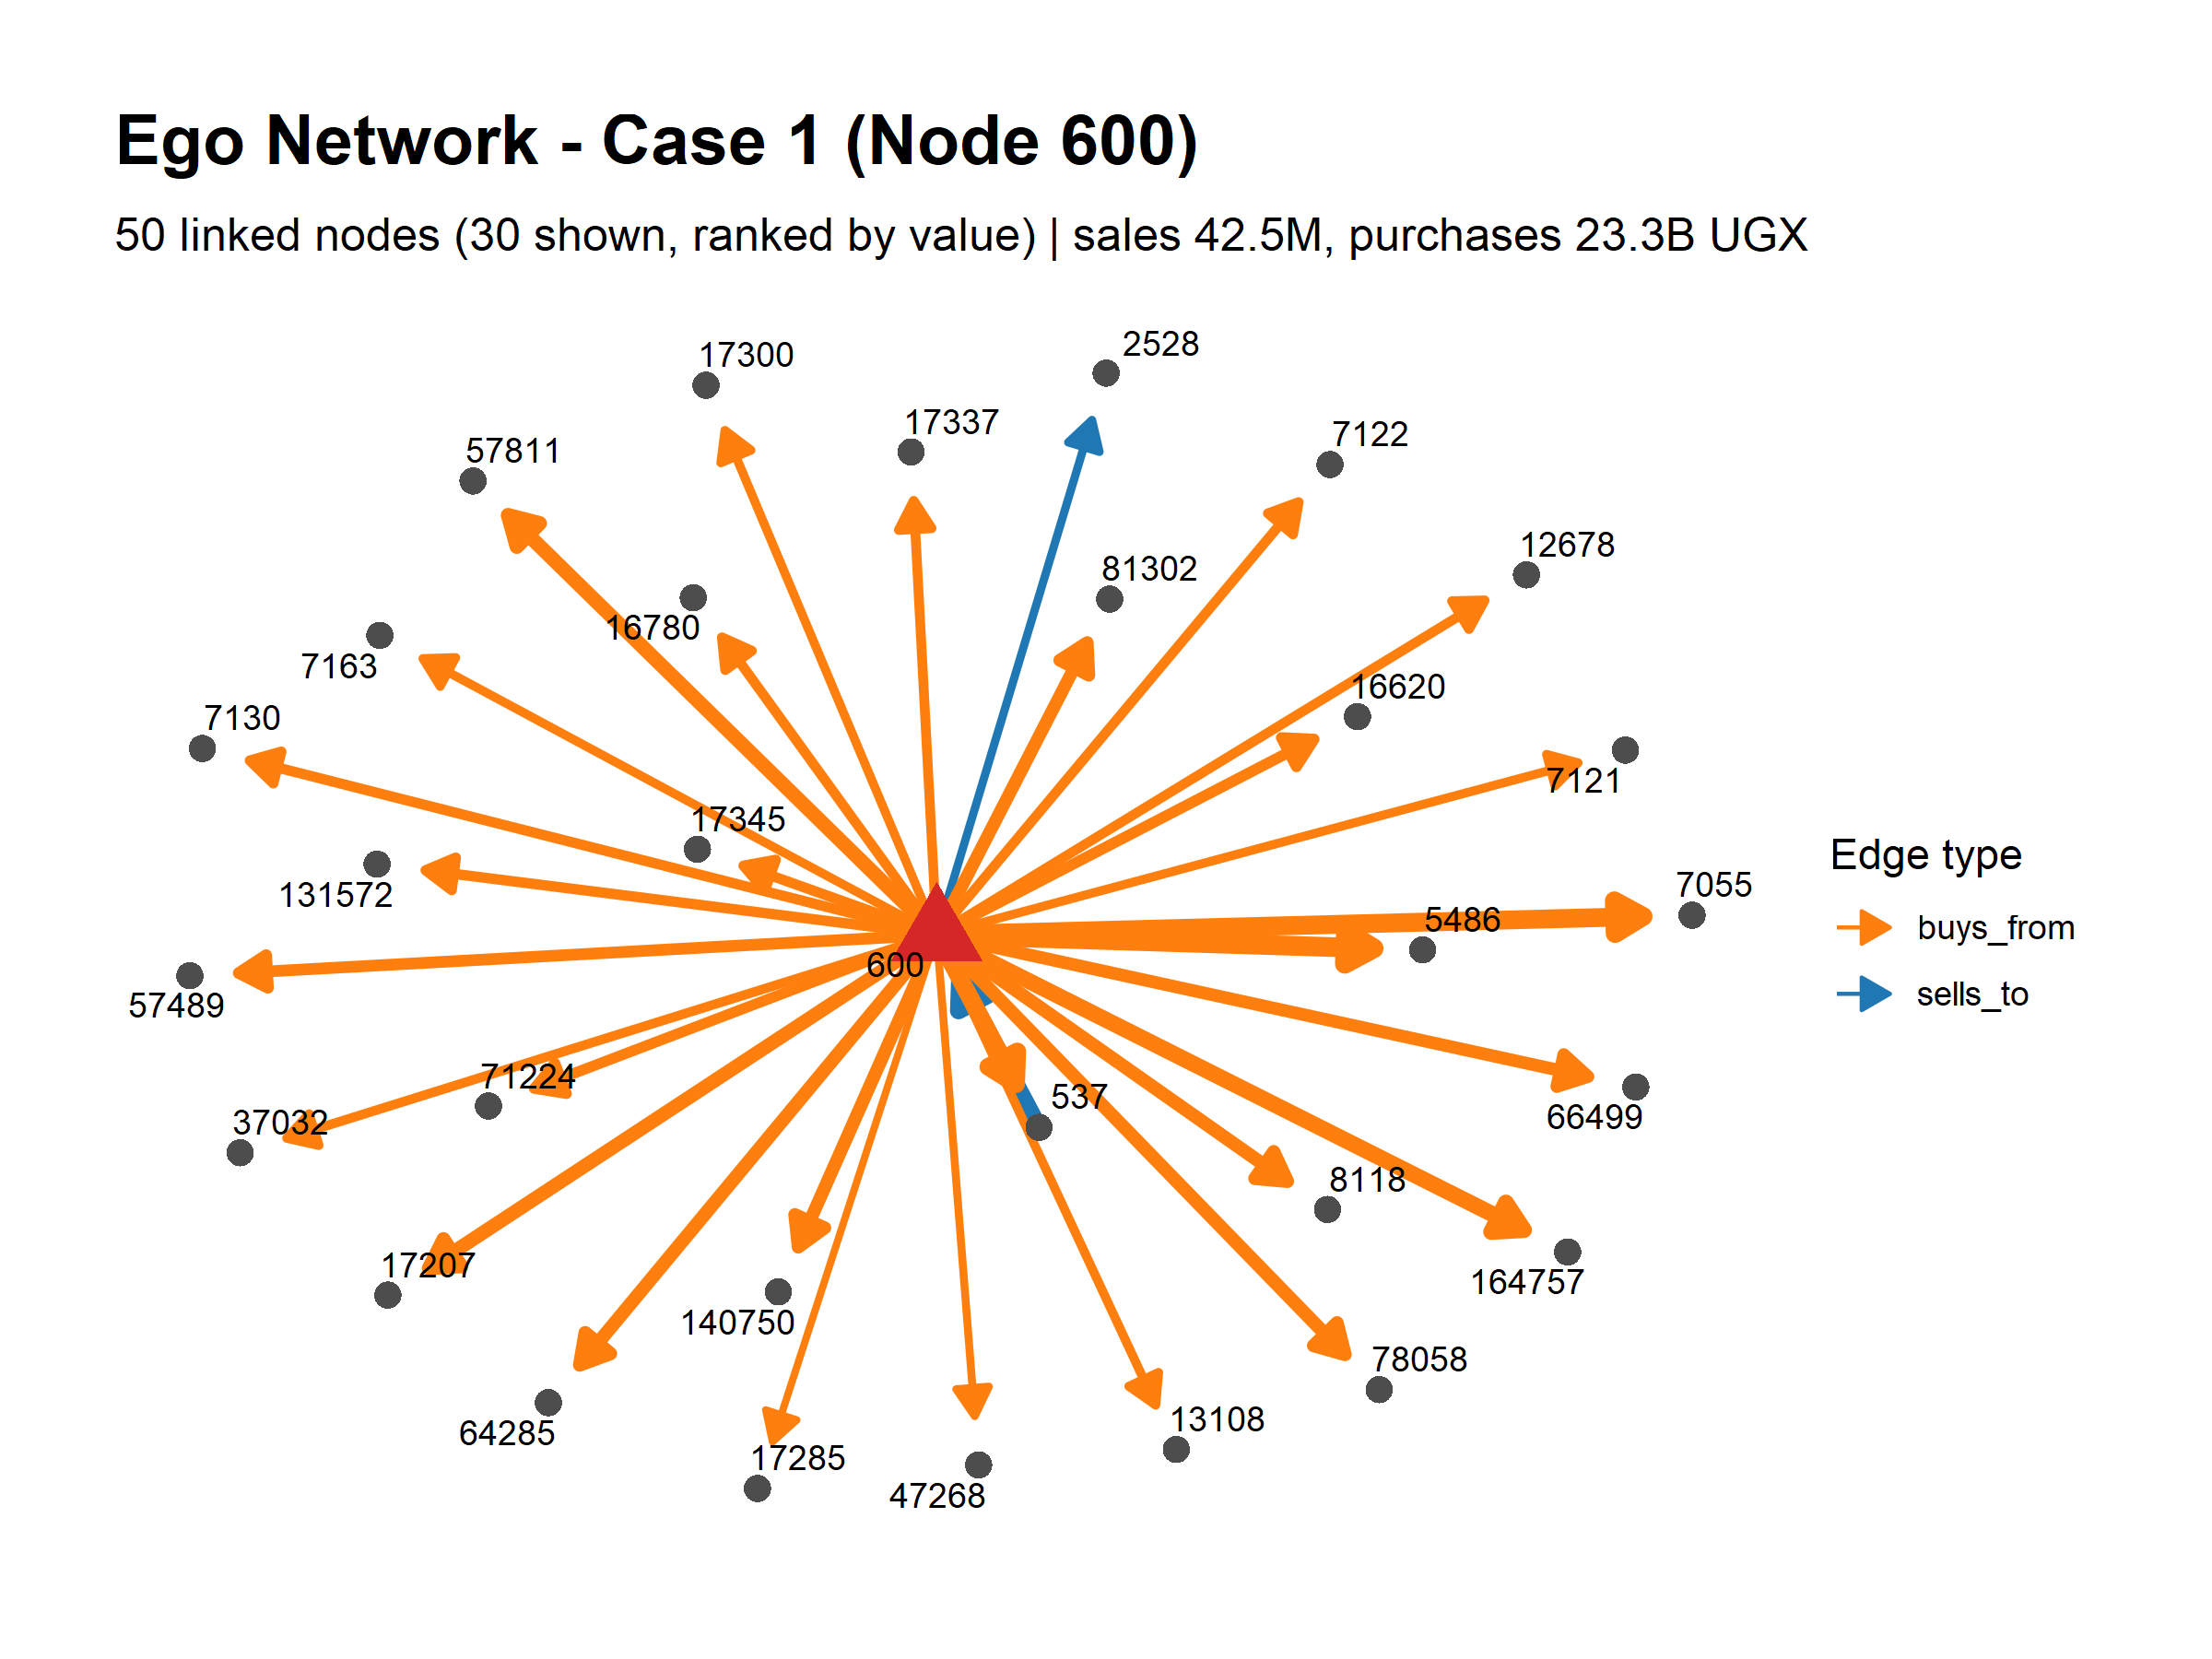
\includegraphics[width=0.85\linewidth]{fig_ego_600.png}
  \caption{Ego network of consensus Node~600, illustrating dense reciprocal interaction with peripheral high-risk suppliers.}
  \label{fig:ego_600}
\end{figure}

\subsection{Longitudinal Filing Dynamics}
Longitudinal analysis indicates that 10 of the 35 consensus taxpayers (28.6\%) exhibited burst activity ($\le 2$ active purchase years over the five-year window), while 25 (71.4\%) exhibited sustained multi-year activity. In the general large taxpayer population, only 11.2\% exhibit burst activity. This 2.6-fold elevation in burst activity among consensus cases aligns with known compliance risk patterns, where shell entities conduct concentrated invoice trading before abandoning registrations.

\subsection{Blinded Auditor Review Set (45 Cases)}
To translate algorithmic candidate leads into operational audit practice and evaluate model discrimination, we constructed a 45-case blinded auditor review set (\texttt{auditor\_review\_blinded.csv}). The set comprises:
\begin{enumerate}
  \item \textbf{35 Consensus Risk Cases:} All corporate taxpayers flagged by two or more independent models (top 10\% cutoff per detector), representing the full actionable output of the multi-model screening pipeline.
  \item \textbf{10 Matched Control Cases:} Non-flagged taxpayers matched to the consensus cohort on visible financial size (total sales and purchases within 1.5 standard deviations in log-space, selected via seed 9413).
\end{enumerate}
The 45 cases are randomized and presented with obscured model labels. This protocol prevents confirmation bias and allows URA risk and audit officers to independently score taxpayer suspicion on a 1--10 scale, establishing Uganda's first structured verification benchmark for graph representation models in revenue administration.

% ============================================================
\section{Policy Implications and Revenue Exposure}
\label{sec:policy}

\subsection{Revenue Exposure Scenarios}
Among the 35 consensus cases, two entities report purchases exclusively with zero downstream sales (Nodes 1554 and 561), accumulating 87.2~million~UGX in invoiced input VAT. Across the wider consensus group, entities displaying severe purchase-to-sales asymmetries represent a combined exposure base of 3,019.8~billion~UGX in invoiced input VAT.

\begin{table}[htb]
  \centering
  \small
  \caption{Potential revenue recovery scenarios across the 3,019.8~billion~UGX input VAT consensus exposure base.}
  \label{tab:revenue}
  \resizebox{\columnwidth}{!}{%
  \begin{tabular}{lcc}
    \toprule
    Scenario & Discrepancy Rate & Potential Exposure \\
    \midrule
    Scenario A (Conservative) & 5\% & 151.0~billion~UGX \\
    Scenario B (Moderate) & 25\% & 754.9~billion~UGX \\
    Scenario C (Aggressive) & 50\% & 1,509.9~billion~UGX \\
    \bottomrule
  \end{tabular}%
  }
\end{table}

Table~\ref{tab:revenue} projects potential revenue exposure under three illustrative audit discrepancy scenarios. Even under the conservative Scenario A (5\% confirmed discrepancy), targeted audits of consensus leads identify an estimated 151.0~billion~UGX in actionable adjustments, exceeding typical random audit yield by several orders of magnitude.

\subsection{Operational Recommendations for URA}
Based on empirical findings, we propose four actionable policy recommendations:
\begin{enumerate}
  \item \textbf{Deploy Automated Baseline Filtering:} Implement a simple automated filter in EFRIS flagging taxpayers reporting $\text{Sales} = 0 \text{ and } \text{Purchases} > \tau$. This filter immediately isolates purchase-only filers at zero computational cost.
  \item \textbf{Institute a Two-Tier Hybrid Architecture:} Pair tabular screening with GNN embedding representations. Taxpayers flagged jointly by tabular and graph detectors (the 35 consensus cases) should receive top priority in the annual Compliance Improvement Plan.
  \item \textbf{Enforce Multi-Seed Ensemble Averaging:} Because raw GAT embeddings exhibit seed initialization variance ($\rho = 0.02 \text{ to } 0.46$), operational deployments must use multi-seed averaging across at least five random initializations prior to case assignment.
  \item \textbf{Build a Verified Ground-Truth Audit Registry:} URA field teams should systematically record audit outcomes for the 35 flagged cases, establishing Uganda's first structured training registry to support future supervised model calibration.
\end{enumerate}

% ============================================================
\section{Discussion and Limitations}
\label{sec:discussion}

This proof-of-concept demonstrates that unsupervised GNNs extract meaningful, orthogonal anomaly signals from real-world administrative e-invoicing data. However, several operational and methodological limitations warrant discussion:
\begin{itemize}
  \item \textbf{Network Boundary Truncation:} The reconstructed graph is bounded by edges incident to the 614 focal large corporate taxpayers. Topological metrics for peripheral counterparties reflect this partial boundary. Full-network graph processing will require distributed graph frameworks.
  \item \textbf{Absence of Verified Historical Ground Truth:} While consensus overlap and synthetic injection validate detector behavior, formal confirmation requires field audit verification by URA compliance officers.
  \item \textbf{Degree Dependence and Seed Stability:} R-GCN link reconstruction error exhibits negative degree correlation ($\rho = -0.39$), requiring degree-normalized scoring. GAT models require multi-seed ensemble aggregation to stabilize stochastic embeddings.
\end{itemize}

Future research will incorporate temporal graph dynamics (such as Temporal Graph Networks \cite{rossi2020temporal}) to capture transient invoice bursts, and explore bipartite line-item commodity graphs to detect cross-commodity invoice fabrication.

% ============================================================
\section{Conclusion}
\label{sec:conclusion}

This study establishes the empirical feasibility of unsupervised Graph Neural Networks for tax anomaly detection using five years of administrative records from Uganda's EFRIS. By reconstructing a multi-relational trade network of 165,094 entities and 471,167 trade links centered on 614 large taxpayers, we demonstrate that self-supervised GNNs uncover complex relational evasion structures that standard tabular models overlook. Augmenting tabular detectors with GAT embeddings elevates circular trading detection from 20\% to 98\% in controlled benchmarks. The 35 consensus anomalies surfaced by our multi-model framework represent 3,019.8~billion~UGX in input VAT exposure, offering high-priority candidate leads for risk-based tax compliance enforcement.

% ============================================================
%  References
% ============================================================
\small
\bibliography{references}

\end{document}
